\def \imgpath {"./figures/colls"}

The aim of this chapter is to give an introduction to the physics of heavy ions and the various phenomena related with the quark-gluon plasma QGP. Furthermore, a detailed summary of the findings of QGP phenomena in small systems, i.e.\ pp and pA collisions, is given. Lastly, some Monte Carlo event generators based on phenomenological modelling of hadronic collisions relevant to this dissertation are summarised.

\section{Collisions of heavy nuclei}

\subsection{Collision geometry, centrality, multiplicity}

Collisions of heavy nuclei, composed of many fluctuating nucleons, may occur under various initial state configurations. Some quantities used to describe them are the impact parameter $b$, defined as the distance between the two nuclei centers, number of participating (scattered) nucleons $\Npart$, and the number of binary nucleonic collisions $\Ncoll$.

Determining these quantities is important because:
\begin{enumerate}
\item Soft processes, such as light flavor particle production, are expected to scale with the interaction volume, which $\propto \Npart$.
\item Hard processes, such as jet and heavy flavor production, are expected to scale with the number of large momentum transfer interactions given by \Ncoll.
\item $b$, disregarding the fluctuations of nucleonic positions, defines the shape and anisotropy of the overlap region, which are important initial state conditions.
\end{enumerate}

Since these quantities cannot be directly measured, they need to be modelled. The charged particle \textit{multiplicity} is commonly used for this purpose, as \meanNch increases monotonically with \Npart, \Ncoll, and decreasing $b$. Multiplicity \Nch can be measured experimentally, e.g.\ with tracking detectors. The concept of \textit{centrality} is also used, which is defined as quantiles of the total nuclear cross-section. For example, a centrality of $0-5\%$ refers to low $b$ values and the top $5\%$ of \Nch values (central events), while $95-100\%$ centrality refers to high $b$ values and the bottom $5\%$ of \Nch values (peripheral events). Centrality can also be inferred from other \textit{event activity} classifiers, such as amplitudes of scintillators at forward rapidity, transverse energy in calorimeters, or energy from beam remnants in zero-degree-calorimeters.

In AA collisions, these relationships are well-defined, and thus the models perform well. The most popular model is the MC Glauber model \cite{millerGlauberModelingHigh2007}. Other models include MC-KLN \cite{kharzeevHadronProductionNuclear2001} and IP Glasma \cite{schenkeFluctuatingGlasmaInitial2012}.

\subsection{MC Glauber model}

The MC Glauber model \cite{millerGlauberModelingHigh2007} takes on a very simple albeit powerful approach. The two nuclei are simulated in three dimensions in a way that satisfies their respective nuclear density profiles, usually modelled by sampling the positions of nucleons from the Woods-Saxon distribution:

\begin{minipage}{0.4\linewidth}
    \begin{center}
        \begin{tikzpicture}
            \draw[->] (-0.25,0) -- (2.5,0) node[right] {$r$};
            \draw[->] (0,-0.2) -- (0,1.2) node[above] {$n(r)$};
            \draw[scale=1,domain=-0.15:2.2,smooth,variable=\x,blue] plot ({\x},{1/(1+exp((\x-1.5)/0.1))});
            \draw[dashed] (1.5,0) node[below] {$R$} -- (1.5,1);
        \end{tikzpicture}
    \end{center}
\end{minipage}%
\begin{minipage}{0.6\linewidth}
    \begin{equation}
        n(r) = \frac{1}{1+\exp((r-R)/a)} \quad ,
    \end{equation}
\end{minipage}

where $R$ is the nuclear radius and $a$ the nuclear skin thickness.

The nucleonic densities can be represented by uniform disks, or more accurately by Fermi-distributions or Gaussian profiles to account for fluctuations of their densities. Their parameters are left free and are tuned to the data.

A random impact parameter is then chosen or sampled. The collision is then treated as a sequence of independent binary nucleon-nucleon collisions, where
\begin{enumerate}
\item nucleons remain travelling in straight lines,
\item the inelastic nucleon-nucleon cross section $\sigma_\mathrm{NN}$ does not depend on the number of interactions,
\item two nucleons are considered to interact if their transverse relative distance $d \leq \sqrt{\sigma_\mathrm{NN}/\pi}$.
\end{enumerate}

Figure~\ref{fig:colls:centrality} illustrates an example of a Glauber Monte Carlo event for a Au+Au collision. By simulating numerous collisions, the average \Npart and \Ncoll are determined\footnote{It also shows the scaling between the numbers of participants and binary collisions, which is approximately $\Ncoll \approx 0.35 \Npart^{4/3}$ .}, and their relations to centrality and event activity observables are determined by fitting to experimental data.

Recent studies have extended the MC Glauber model to include sub-nucleonic structures. Such efforts show that the production of charged hadrons at mid-rapidity scales linearly with the number of participating partons. Comparisons with LHC data at \snnt{5.02} suggest that the number of sub-nucleonic degrees of freedom ranges from $3$ to $5$ \cite{loizidesGlauberModelingHighenergy2016}.

\begin{figure}[H]
\subfloat[][]{\adjustbox{valign=m}{\adjincludegraphics[trim={{.33\width} 0 {.33\width} 0},clip,width=.29\textwidth]{\imgpath/glauber_mc_event.pdf}}}\hspace{2em}
\subfloat[][]{\adjustbox{valign=m}{\includegraphics[width=.490\textwidth]{\imgpath/cocktail3.eps}}}
\caption{\textbf{(a)} Glauber Monte Carlo event of a Au+Au collision at \snng{200} shown in the transverse plane (top panel) and along the beam axis $z$ (bottom panel). The darker circles represent participating nuclei and their area corresponds to $\sigma_\mathrm{NN}$. \textbf{(b)} Illustrative diagram of the dependence of final-state event multiplicity on the initial-state quantities, number of participants \Npart and impact parameter $b$. \cite{millerGlauberModelingHigh2007}}
\label{fig:colls:centrality}
\end{figure}

\section{Quark-gluon plasma}

In agreement with lattice QCD predictions \cite{borsanyiThermodynamicsQCDTransition2013}, the QGP has been measured in ultra-relativistic collisions of heavy nuclei at RHIC \cite{arseneQuarkGluonPlasma2005, adamsExperimentalTheoreticalChallenges2005}, LHC \cite{niidaSignaturesQGPRHIC2021}, and even SPS \cite{heinzEvidenceNewState2000}. Although it cannot be observed directly, a wealth of evidence from three decades of research combining various observables reveals the effects of the produced QGP medium. Whilst somewhat context-dependent, the following features make QGP the most extreme phenomenon observed in terms of its:
\begin{itemize}
\item \textit{Temperature}: QGP temperatures reach values on the order of hundreds of MeV, which corresponds to approximately $2 \times 10^{12}$~K.\footnote{Contrasting some of the lowest temperatures required for the super-conducting magnets of the LHC, $T \approx 1.9$~K.} \cite{cmscollaborationMeasurementNuclearModification2019}
\item \textit{Viscosity}: the shear viscosity to entropy density ratio $\eta/s$ reaches the minimum quantum limit of $1/4\pi$ (for water at room temperature, $\eta/s \approx 8$), making it an almost perfect liquid. \cite{pasechnikPhenomenologicalReviewQuark2017}
\item \textit{Vorticity}: in semi-peripheral collisions, the rotating plasma reaches a vorticity of approximately $9\times 10^{21}$ s$^{-1}$. \cite{adamczykGlobalHyperonPolarization2017}
\item \textit{Magnetic field}: in non-central collisions, the magnetic fields in the system may peak at $\sim 10^{19}$ T. \cite{kharzeevEffectsTopologicalCharge2008}
\end{itemize}

\begin{figure}[H]
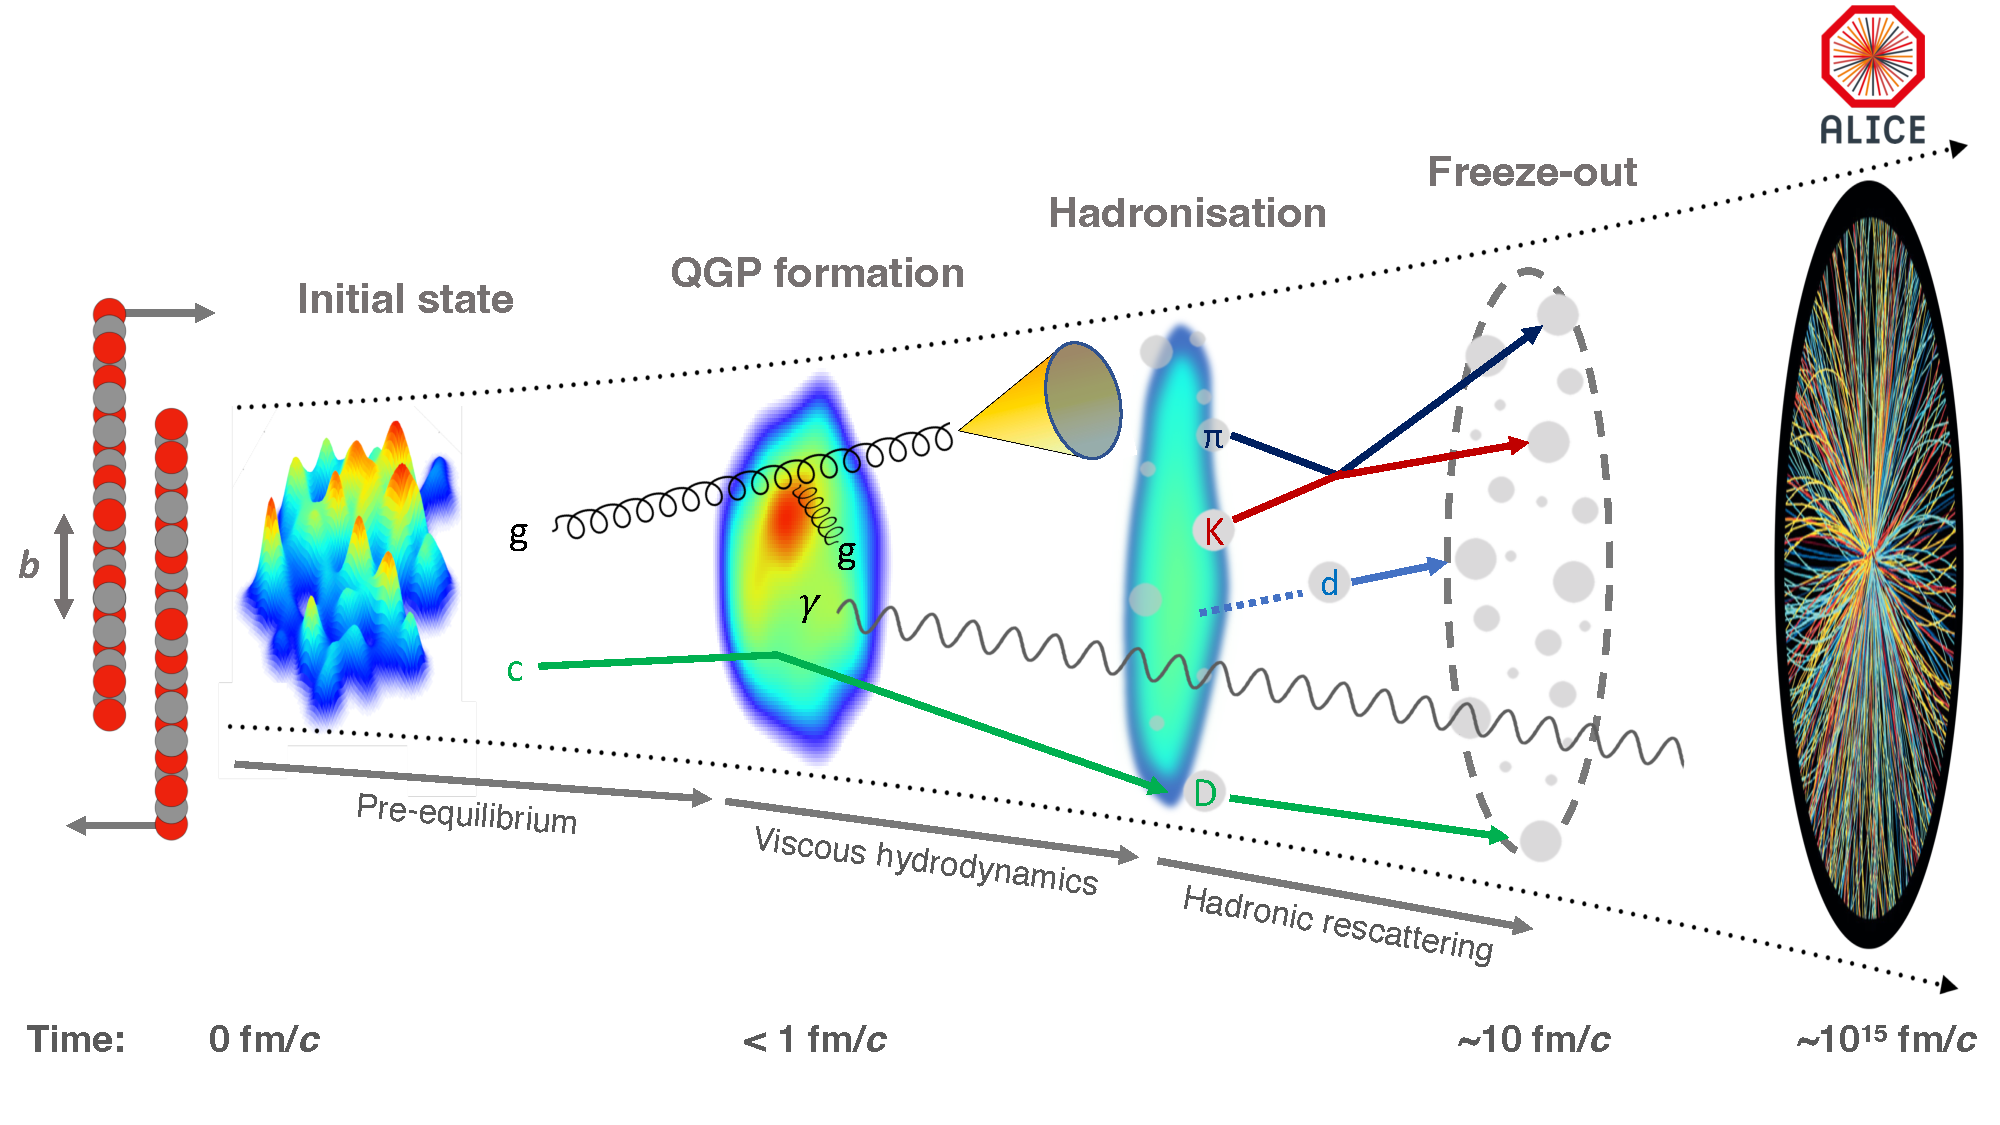
\includegraphics[width=.90\textwidth]{\imgpath/evolution.pdf}\\
\caption{Evolution of heavy nuclei collisions at LHC energies, depicting the different stages. \cite{alicecollaborationALICEExperimentJourney2022}}
\label{fig:colls:evolution}
\end{figure}

Figure~\ref{fig:colls:evolution} illustrates the common paradigm for the different stages of a collision between heavy nuclei:
\begin{enumerate}
\item The Lorentz-contracted heavy nuclei approach each other at ultra-relativistic speeds.
\item \textit{Pre-hydrodynamisation stage} ($\tau \equiv \sqrt{t^2 - z^2} \leq 1$ fm/c): ``hard" particles are produced in scatterings with the highest momentum transfer $Q^2$. Produced matter expands rapidly in the longitudinal direction and starts expanding in the radial direction.
\item \textit{Hydrodynamisation} ($1 \leq \tau \leq 10$ fm/c): abundantly produced partons create a deconfined medium, which can be described by hydrodynamic equations.
\item \textit{Chemical freeze-out} ($\tau \sim 10$ fm/c): the system cools down and hadronises. The produced hadrons then stop interacting inelastically and the system's chemical content is stabilised.
\item \textit{Kinetic freeze-out} ($\tau \lesssim 20$ fm/c): hadrons no longer interact elastically and their kinematics stabilize.
\item Long-lived particles can be measured in the detector volume. 
\end{enumerate}

The following subsections outline some of the essential phenomena related to the production of QGP.

\subsection{Quarkonium dissociation and sequential suppression}

Heavy quarkonia are vector meson states consisting of $c\bar{c}$ and $b\bar{b}$. They include $J/\psi$, $\psi(2\mathrm{S})$, $\Upsilon(1\mathrm{S})$, $\Upsilon(2\mathrm{S})$, $\Upsilon(3\mathrm{S})$, which can be relatively easily measured in LHC experiments via their di-lepton decay channels. They are created solely in the first phases of the collision and then experience the entire evolution of the QGP medium:
\begin{equation}
t^{Q\overline{Q}}_\mathrm{creation} < t^\mathrm{QGP}_\mathrm{creation} < t^\mathrm{QGP}_\mathrm{lifetime} \ll t^{Q\overline{Q}}_\mathrm{lifetime} \quad .
\end{equation}

Additionally, due to their large binding energies, their radii may remain smaller than the plasma screening radius $r_\mathrm{D}(T)$, and thus, survive the dissociation. For instance, considering their in-vacuum radii determined from the $q\bar{q}$ potential, $r_{\Upsilon(1\mathrm{S})}\sim 0.14$~fm, $r_{\Upsilon(2\mathrm{S})}\sim 0.28$~fm, $r_{\Upsilon(3\mathrm{S})}\sim 0.39$~fm, which contrast the $r_\pi \sim 0.7$~fm \cite{sarkarPhysicsQuarkGluonPlasma2010}. This implies that different temperatures result in the dissociation of different states, and measuring the production of different states can help infer the QGP temperature, as illustrated in Fig.~\ref{fig:colls:thermometer} \cite{matsuiSuppressionQuarkgluonPlasma1986, satzProbingStatesMatter2013}.

\begin{figure}[H]
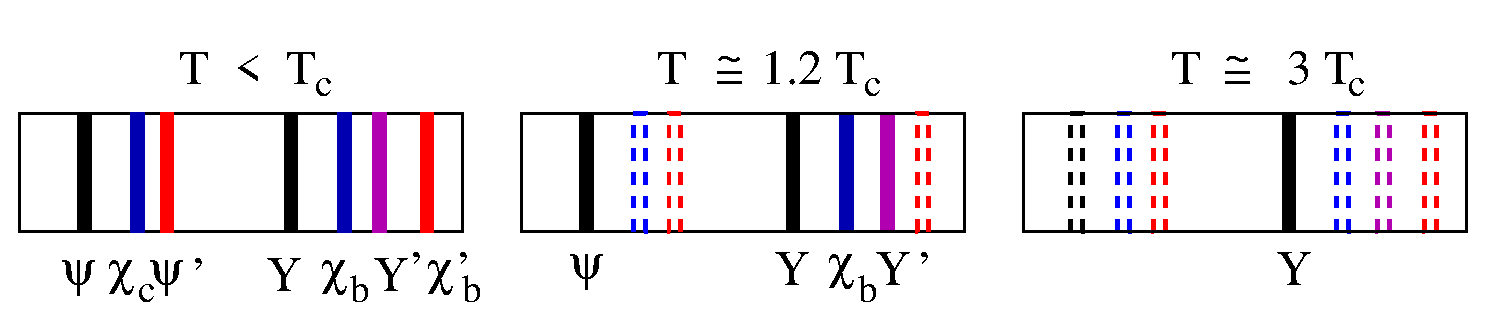
\includegraphics[width=.70\textwidth]{\imgpath/spec.eps}
\caption{Spectral lines corresponding to various charmonium and bottomonium states for different medium temperatures , relative to the QGP critical temperature. \cite{satzProbingStatesMatter2013}}
\label{fig:colls:thermometer}
\end{figure}

The production of heavy quarkonia in AA collisions is compared to that in pp collisions (scaled by the average number of binary collisions) through the nuclear modification factor, $R_{\mathrm{AA}}$. This quantity is widely used in various other measurements and is defined as:
\begin{align}
R_{\mathrm{AA}}=\frac{\mathrm{d}N_{\mathrm{AA}}/\mathrm{d}\pt}{\langle N_{\mathrm{coll}}\rangle\ \mathrm{d}N_{\mathrm{pp}}/\mathrm{d}\pt} \quad .
\end{align}
$R_{\mathrm{AA}}$ can take on the following values:
\begin{enumerate}
\item $R_\mathrm{AA} = 1$: The result one would expect if the AA collision is a mere superposition of nucleon-nucleon collisions. There is no net effect on the production, corresponding to the absence of the QGP medium and other nuclear effects, or their mutual cancellation.
\item $R_\mathrm{AA} < 1$: The production is overall suppressed, for example, due to dissociation.
\item $R_\mathrm{AA} > 1$: The plasma and nuclear effects systematically enhance the measured production.
\end{enumerate}

At LHC energies, the abundance of charm quarks in the QGP is high enough that charmonia can be formed after dissociation, which somewhat complicates the interpretation of charmonia suppression. However, the $\Upsilon(3\mathrm{S})$ bottomonium has $R_{\mathrm{AA}}$ consistent with zero at $\sqrt{s_{\mathrm{NN}}}=5.02$ TeV, as shown in Fig.~\ref{fig:colls:cmsupsilon} \cite{cmscollaborationMeasurementNuclearModification2019}. This complete suppression is a clear signature of the QGP and can be used together with models to estimate the QGP temperature at these energies as $T\approx 630$~MeV \cite{krouppaPredictionsBottomoniaSuppression2016}.

\begin{figure}[H]
\subfloat[][]{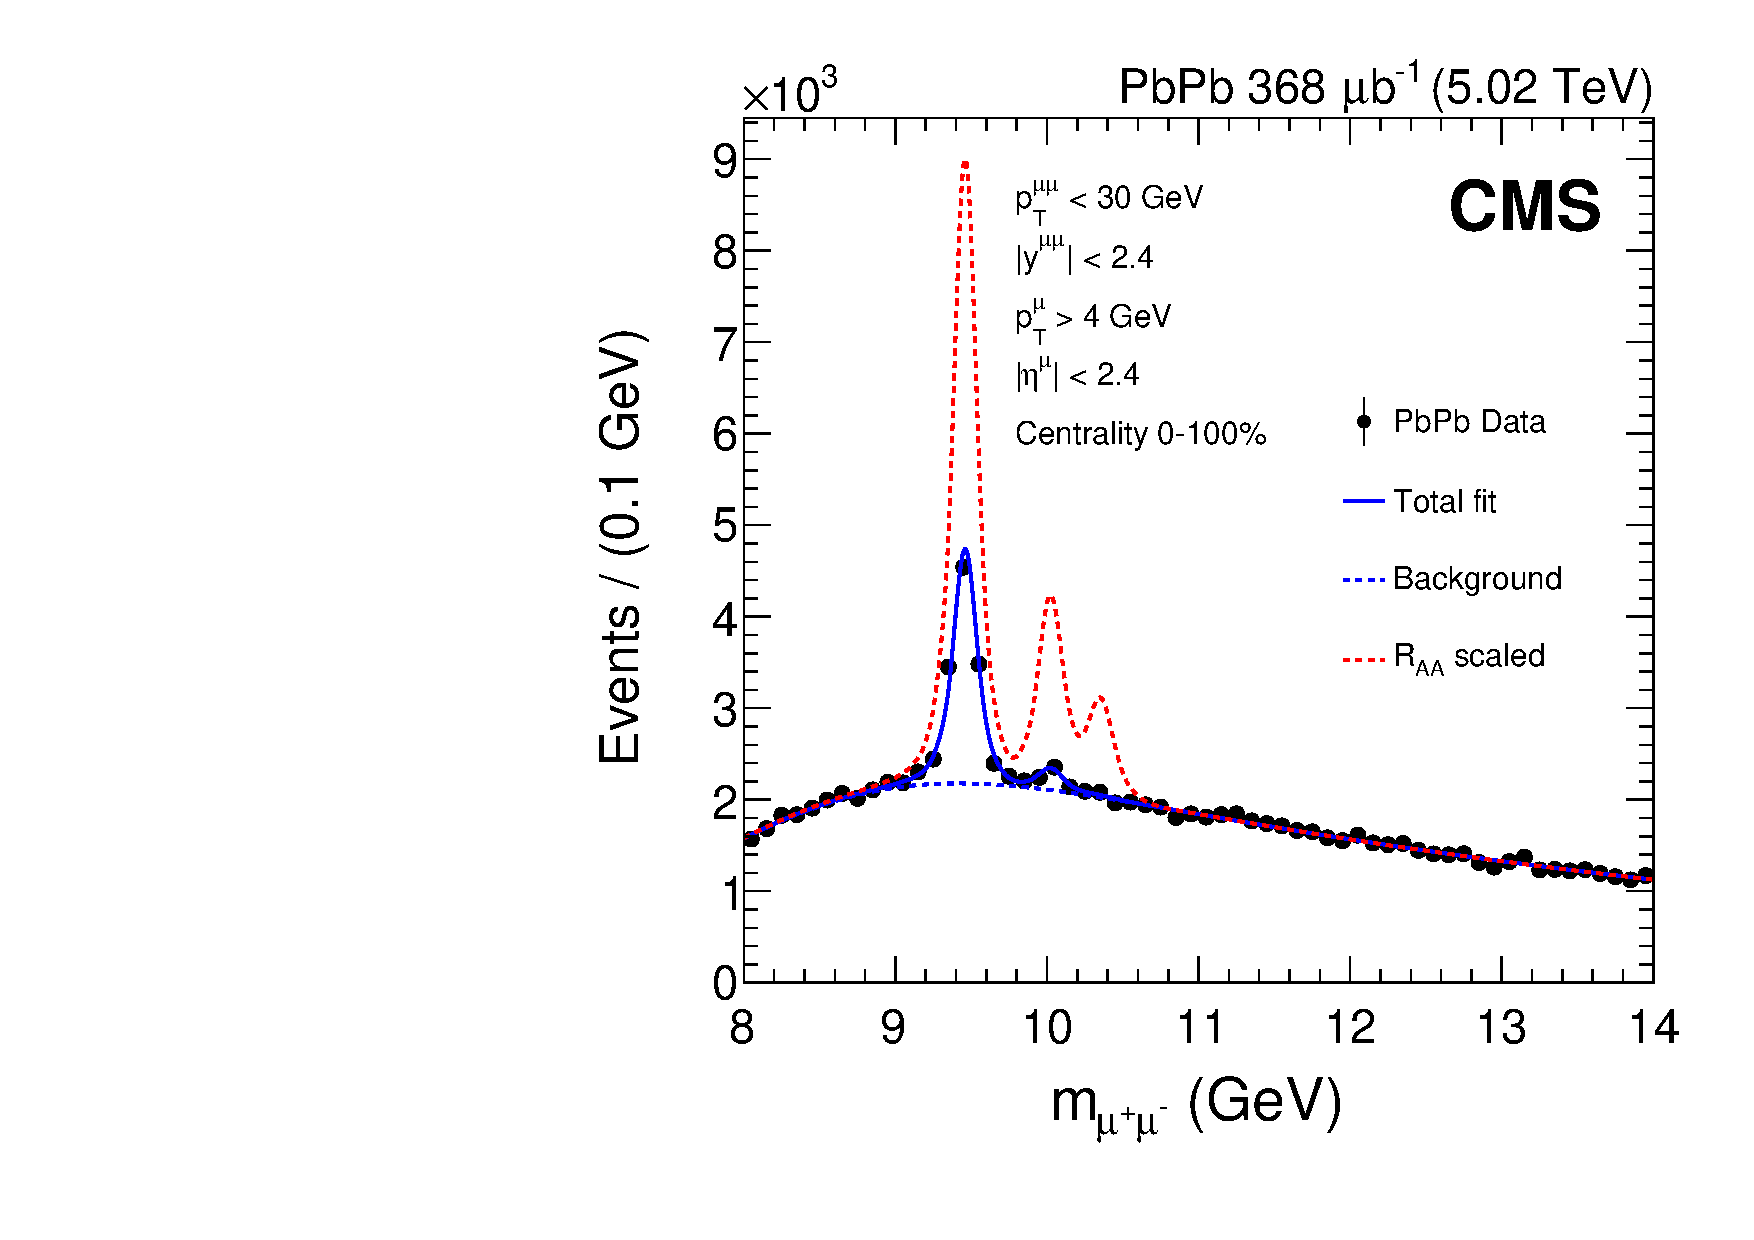
\includegraphics[width=.40\textwidth]{\imgpath/cms_ups1.pdf}}\hspace{2em} 
\subfloat[][]{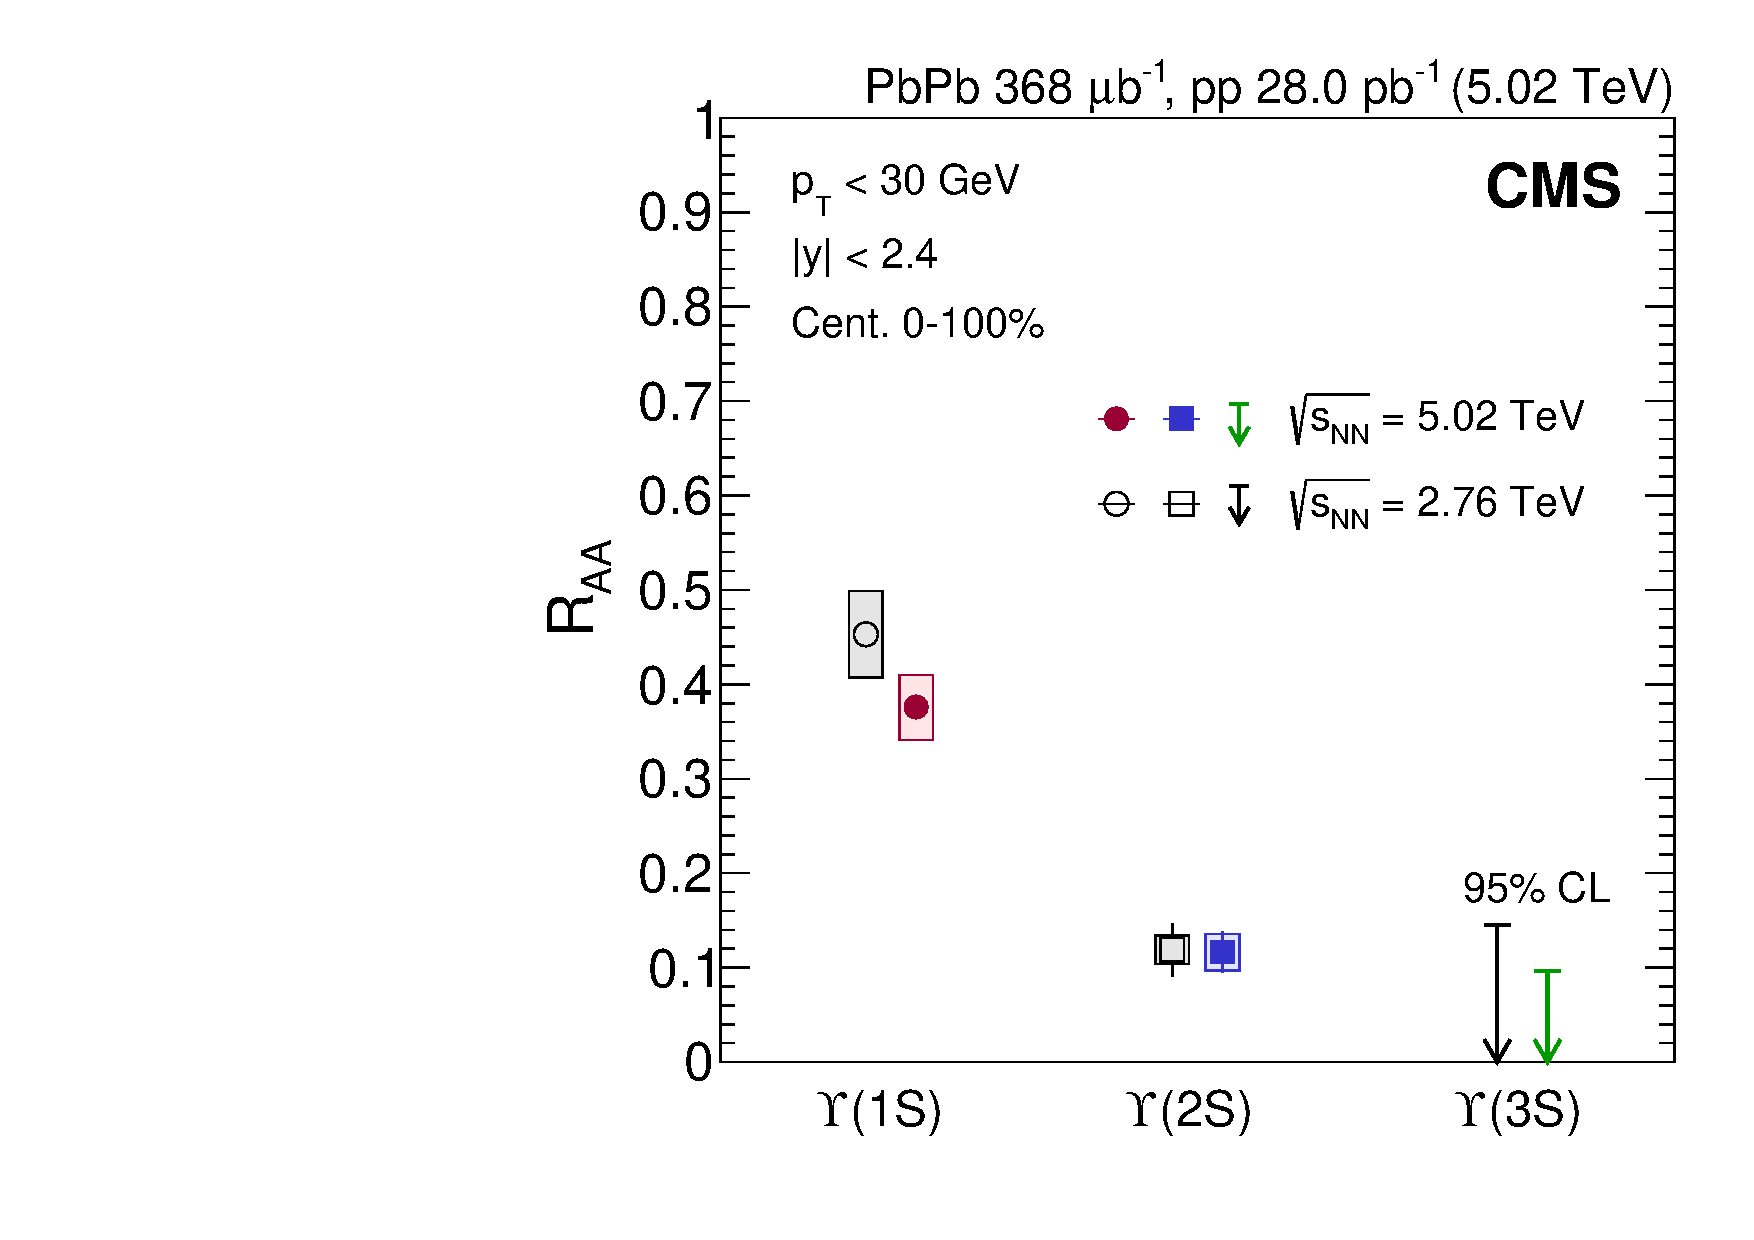
\includegraphics[width=.41\textwidth]{\imgpath/cms_ups2.pdf}}
\caption{\textbf{(a)} Muon invariant mass distributions in Pb-Pb collisions at \snnt{5.02}, also showing a scaled result from pp collisions at same energies (red dashed line). \textbf{(b)} Nuclear modification factors of the three bottomonium states. \cite{cmscollaborationMeasurementNuclearModification2019}}
\label{fig:colls:cmsupsilon}
\end{figure}

\subsection{Strangeness enhancement}

In the production of hadrons in vacuum, strangeness is suppressed relatively to light quarks not only due to the higher mass of the strange quark ($m_s \approx \gevcc{0.1}$), but also due to the much higher constituent mass ($m_K \approx \gevcc{0.5}$). However, in the QGP, due to the high gluon densities and $T\sim m_s$, strangeness production may equilibrate with $u$ and $d$ quarks through gluon fusion:
\begin{align*}
gg \to s\bar{s} \quad .
\end{align*}

This phenomenon was proposed as one of the first signatures of QGP observation in colliders \cite{rafelskiStrangenessProductionQuarkGluon1982, kochStrangenessRelativisticHeavy1986}. Indeed, an enhancement in the production of strange hadrons is observed in AA collisions, which is dependent on the event activity and increases with increasing strangeness content of the hadron \cite{alicecollaborationMultistrangeBaryonProduction2016}. Figure~\ref{fig:colls:strangeness} displays these results.

Furthermore, the yields of hadrons measured in AA collisions can be accurately described by statistical models \cite{andronicThermalHadronProduction2009, wheatonTHERMUSThermalModel2009} which, generally, assume that the dense system is in thermal and chemical equilibrium at the point of its freeze-out. In these models, strangeness is assumed to be conserved on average, which corresponds to a grand-canonical ensemble with a strange chemical potential $\mu_S$. 

In small systems, the conservation of strangeness must be taken into account for each interaction, locally. This necessitates the use of a canonical ensemble and introducing a parameter, $V_0$, to describe the volume of this locality requirement \cite{hamiehCanonicalDescriptionStrangeness2000}. With this approach, strangeness enhancement can be reproduced by increasing $V_0$ and transitioning from the canonical ensemble in small systems to the grand-canonical ensemble in AA collisions, as depicted in Fig.~\ref{fig:colls:strangeness}.

\begin{figure}[H]
\subfloat[][]{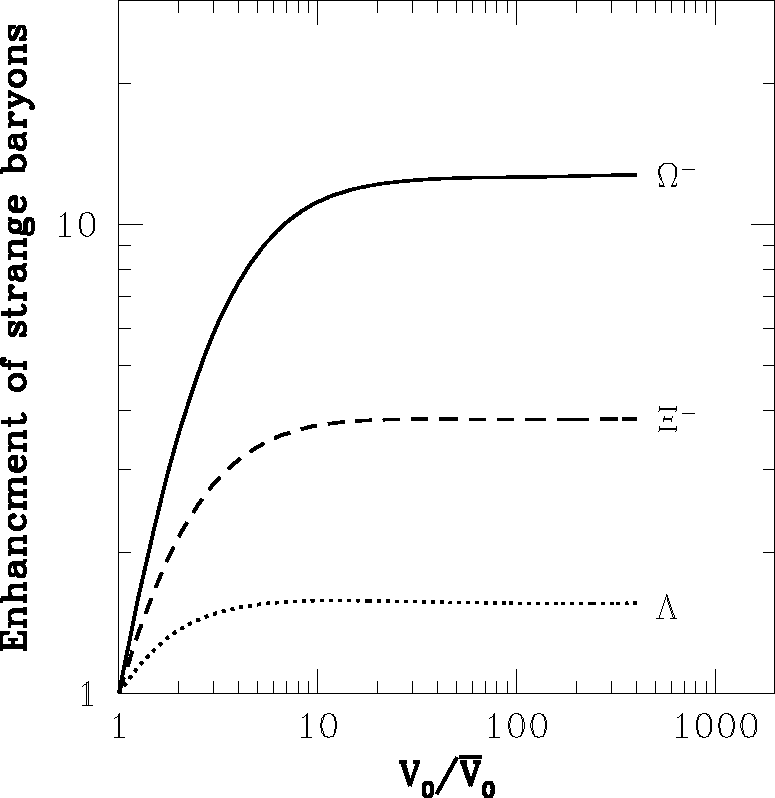
\includegraphics[height=11.85em]{\imgpath/se_v02.pdf}}\hspace{1em}
\subfloat[][]{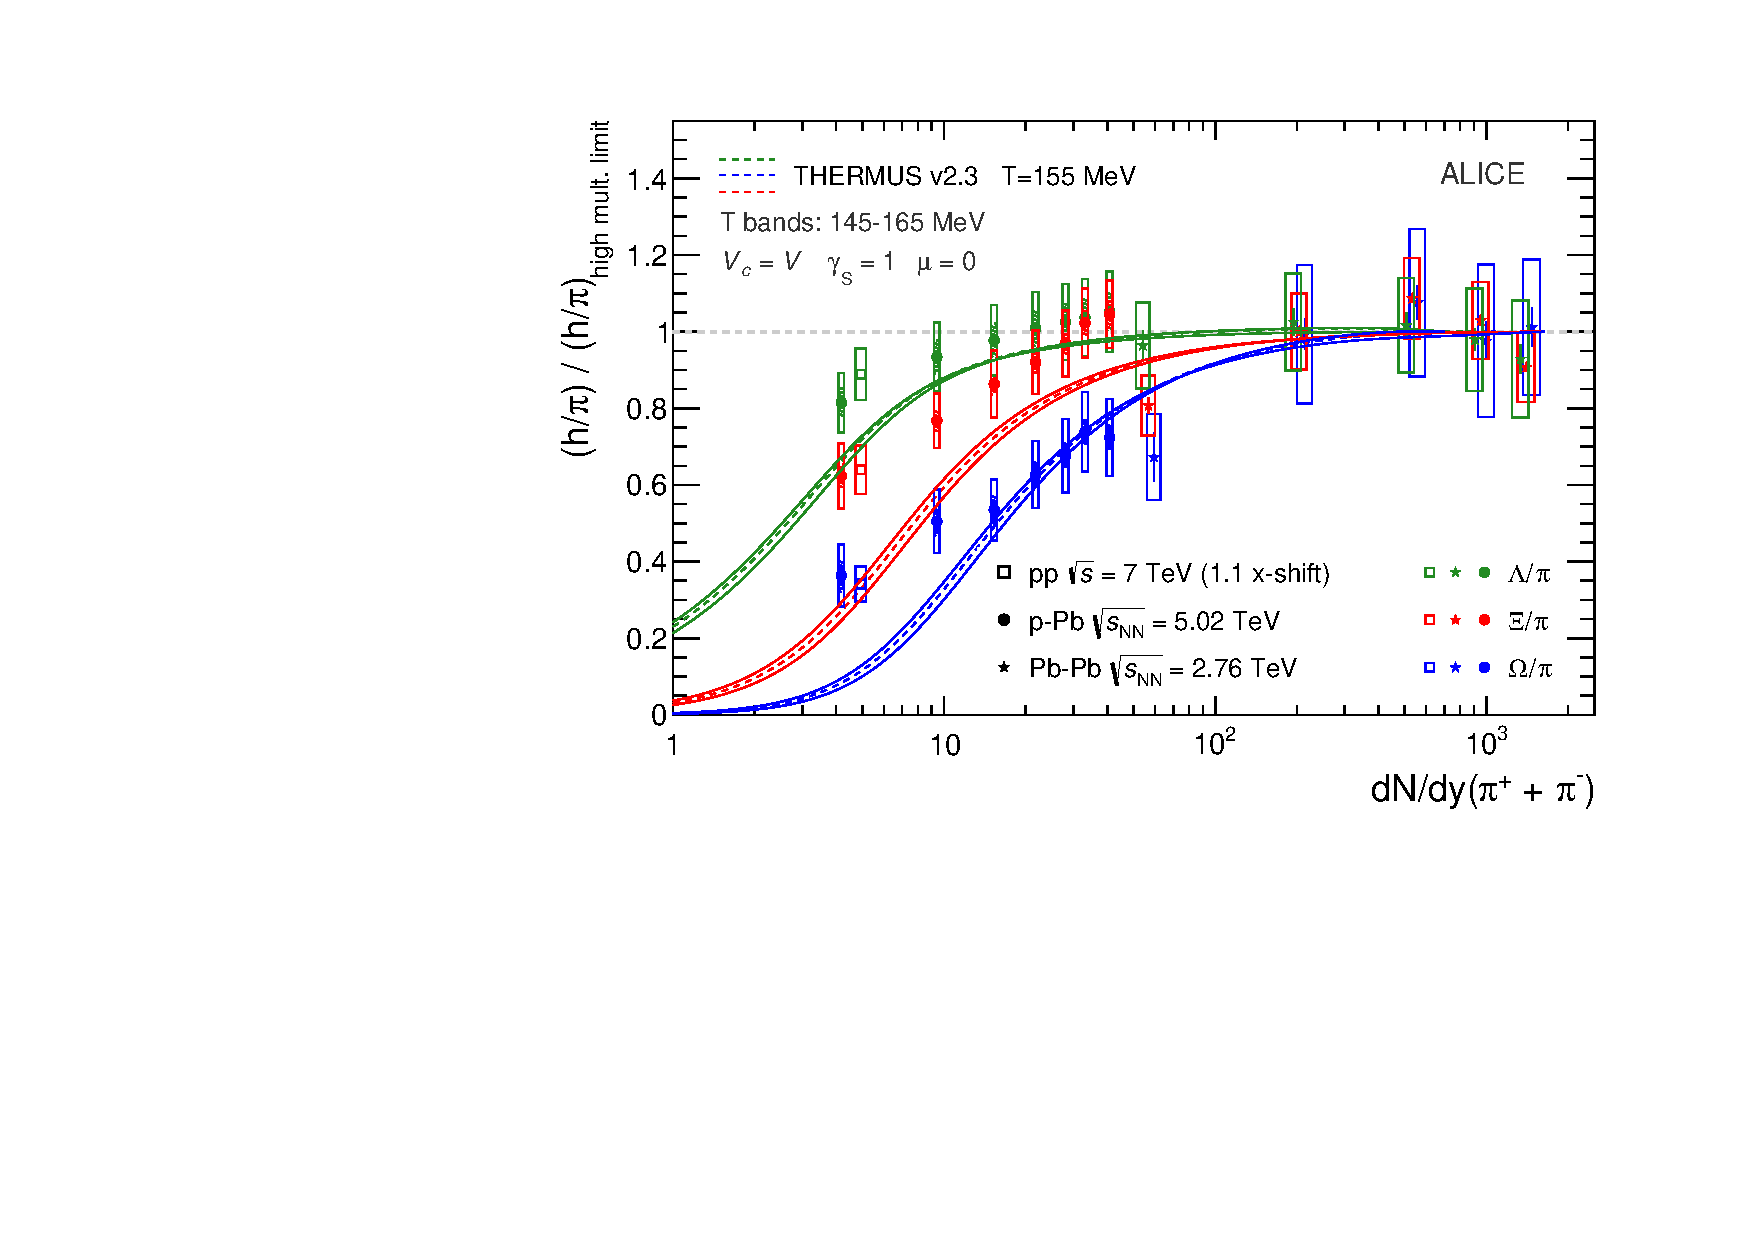
\includegraphics[height=13em]{\imgpath/se_omegaxi.pdf}}
\caption{\textbf{(a)} Dependence of strange baryon densities on the parameter $V_0$ characterising the volume where strangeness is locally conserved in models describing strangeness suppression in small systems as canonical suppression. The volume is normalised to a typical AA value of $\overline{V}_0=7.4$~fm$^{3}$. \cite{hamiehCanonicalDescriptionStrangeness2000}. \textbf{(b)} Ratios of yields of strange baryons to pions in pp, p-Pb, and Pb-Pb collisions as a function of the pion multiplicity normalised to the high-multiplicity limit in $0-60\%$ most central Pb-Pb collisions. The results are compared with a statistical model combining the canonical and grand-canonical approach. \cite{alicecollaborationMultistrangeBaryonProduction2016, wheatonTHERMUSThermalModel2009}}
\label{fig:colls:strangeness}
\end{figure}

%\begin{figure}[H]
%\subfloat[][]{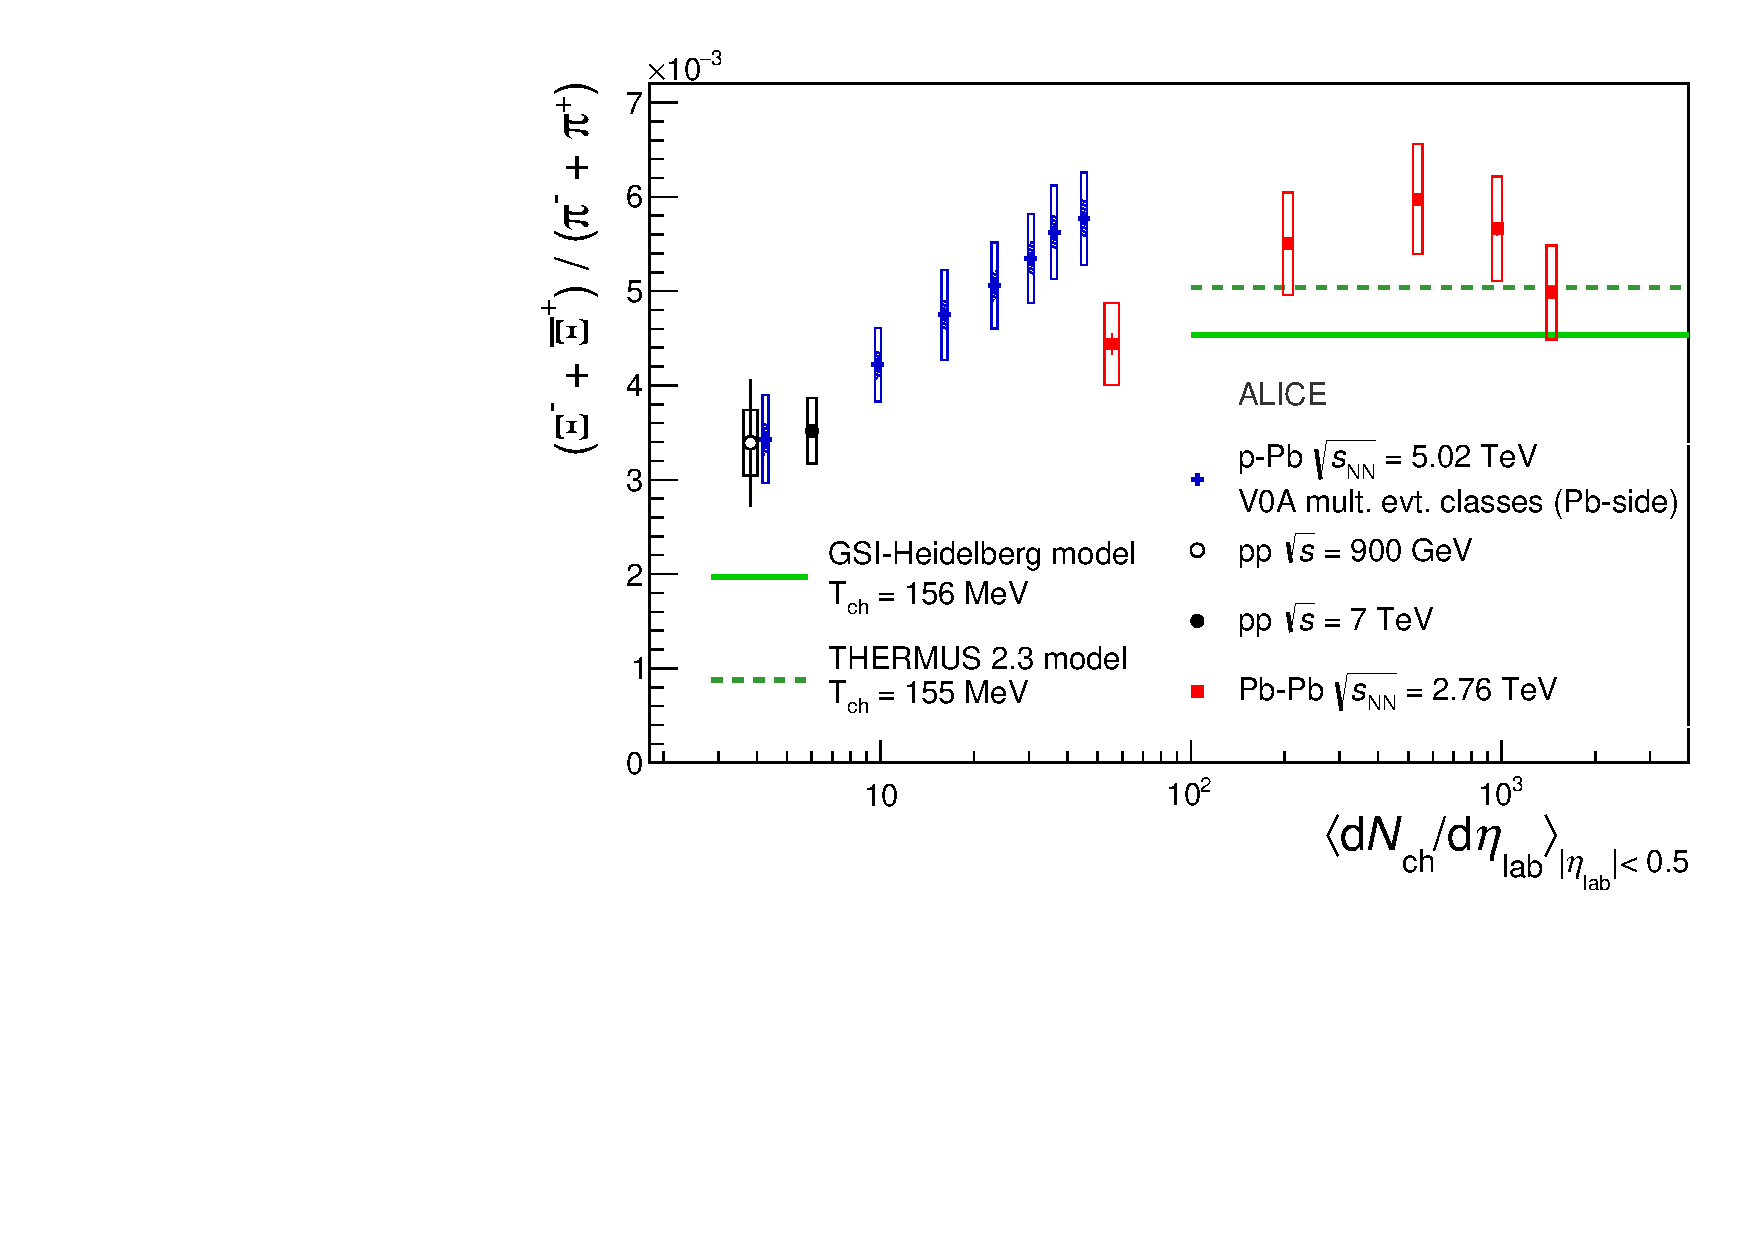
\includegraphics[width=.47\textwidth]{\imgpath/xitopi.pdf}}\hspace{1em}
%\subfloat[][]{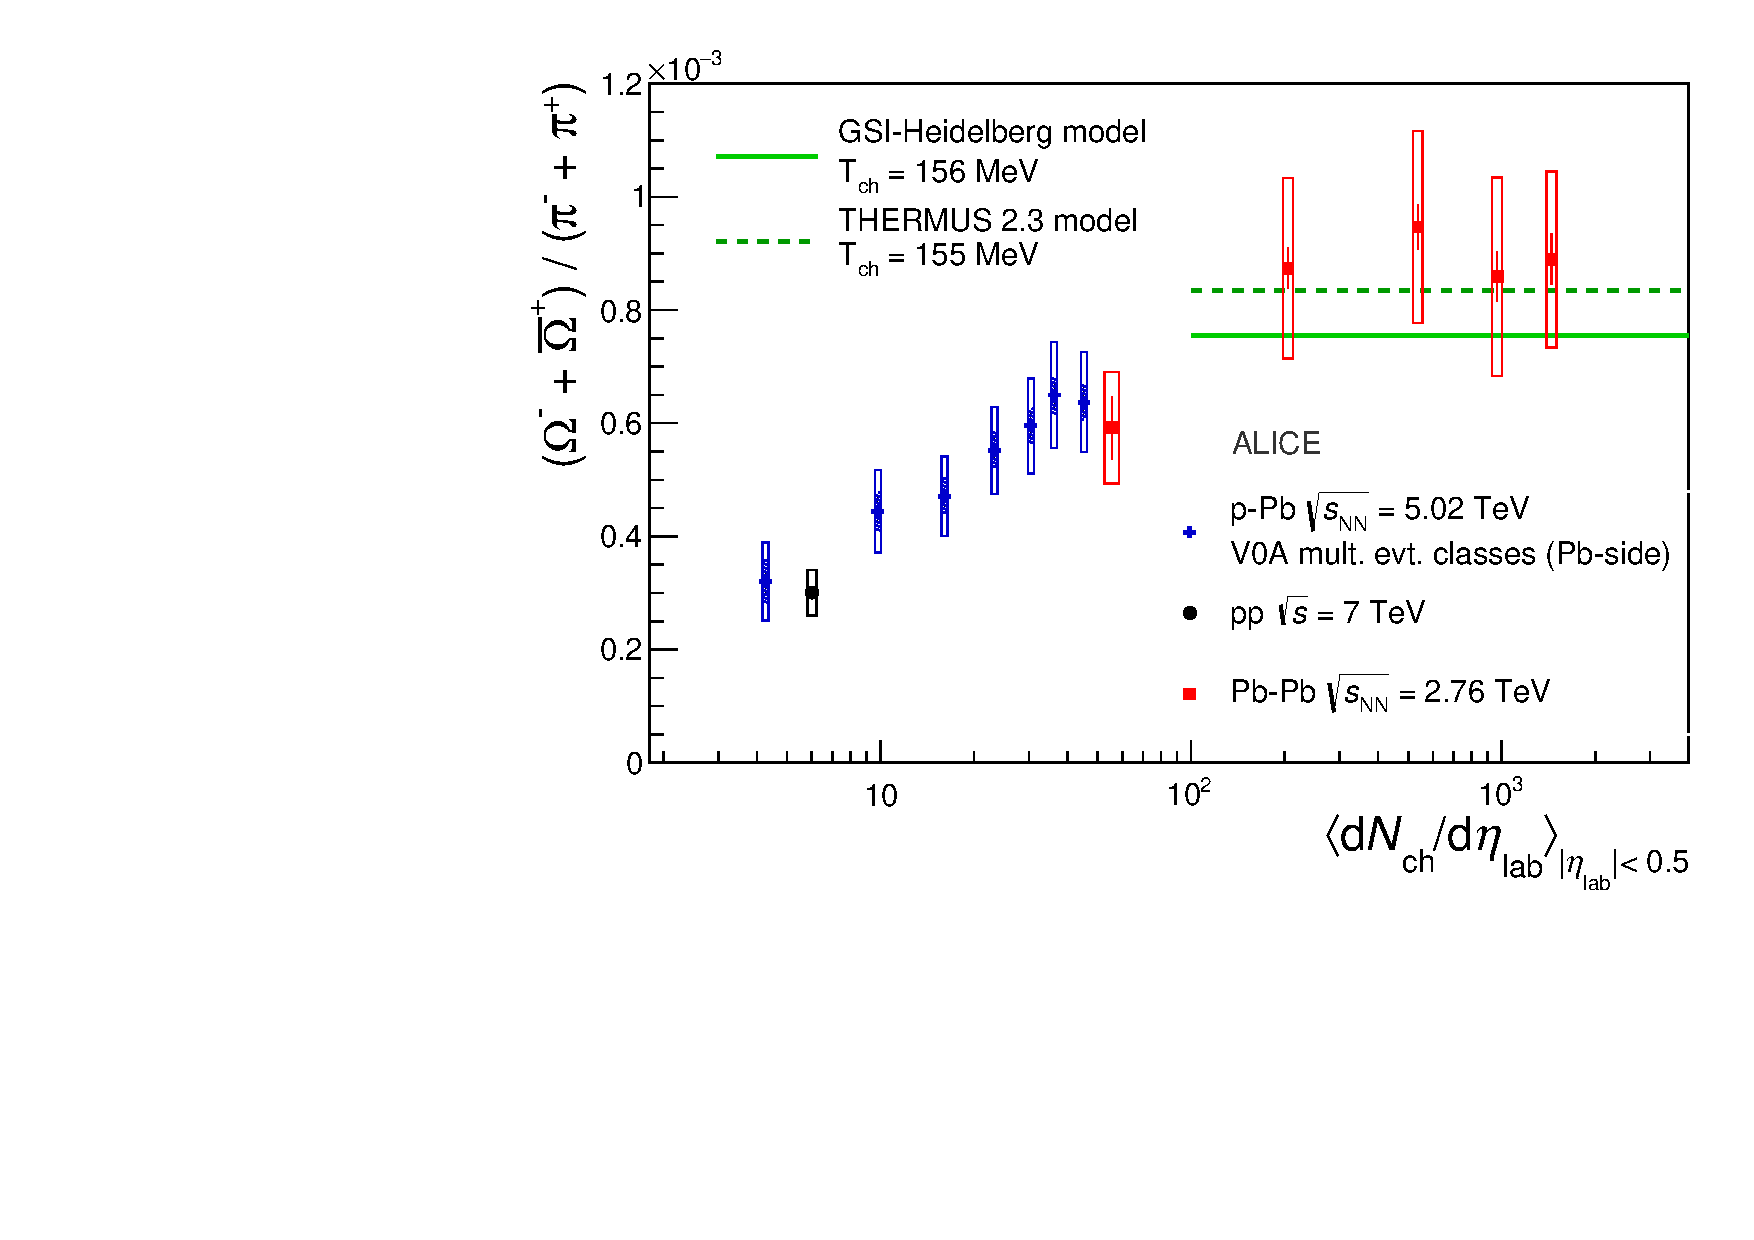
\includegraphics[width=.47\textwidth]{\imgpath/omegatopi.pdf}}
%\caption{TBA}
%\label{fig:colls:strangeness}
%\end{figure}

\subsection{Collective flow}

The strongly interacting plasma exhibits a collective expansion which can be described by hydrodynamic equations, since the mean free paths of the constituents are much smaller than the system size ($\lambda \ll L$). The non-uniform energy density in the initial state results in varying pressure gradients, which drive this expansion. Since the centre of the plasma has greater pressure than its outside regions, common expansion velocity field develops, which results in the so-called \textit{radial flow}. Similarly, the medium also translates the directionally-dependent anisotropies in the initial state, which stem from the almond-shape geometry of the collision overlap region as well as nucleonic fluctuations, to the final-state. This is the so-called \textit{anisotropic flow}.

Together with hadronic re-scattering, the flows are reflected in the kinematics of the final-state hadrons. When comparing \pt spectra in central AA collisions to those in peripheral or in pp collisions, a broadening as well as a momentum boost can be observed (see Fig.~\ref{fig:colls:rflow}), caused by the radial expansion as well as the less important thermal motion \cite{alicecollaborationCentralityDependenceRm2013, alicecollaborationRmSRm2013, alicecollaboration8920Phi2015}. The expansion effect depends on the mass of the hadrons, as the amount of additional \pt acquired is proportional to their mass and the collective expansion velocity field, $p \approx m\beta c$. A notable exception to this trend is the $\phi$ quarkonium; although comparable with the proton ($m_\phi \approx \gevcc{1.02} \sim m_p$), its scattering cross-section is much smaller \cite{hungEquationStateRadial1998}.

The \pt spectra influenced by radial flow can be described by the Blast-Wave parametrisation \cite{schnedermannThermalPhenomenologyHadrons1993}. In this approach, the radial expansion is accounted for as a common velocity field profile $\beta (r)$ affecting thermal spectra, 

\begin{minipage}{0.5\linewidth}
    \begin{center}
        \begin{tikzpicture}
            \draw[->] (-0.25,0) -- (2.5,0) node[right] {$r$};
            \draw[->] (0,-0.2) -- (0,1.2) node[above] {$\beta(r)$};
            \draw[scale=1,domain=0.0:2.2,smooth,variable=\x,blue] plot ({\x},{0.95*(\x/2.2)^0.7});
            \draw[dashed] (2.2,0) node[below] {$R$} -- (2.2,1);
        \end{tikzpicture}
    \end{center}
\end{minipage}%
\begin{minipage}{0.5\linewidth}
    \begin{equation}
		\beta (r) = \beta_s (\frac{r}{R})^n \quad ,
    \end{equation}
\end{minipage}

where $\beta_s$, $R$, and $n$ are the expansion velocity on the surface of the plasma, its radius, and an extra parameter usually ranging $0.7-1.0$ in central collisions \cite{alicecollaborationCentralityDependenceRm2013}, respectively. The effects of radial flow can also be reproduced in AA collisions with hydrodynamic models using an equation of state from LQCD and hadronic re-scattering \cite{hungEquationStateRadial1998}, and in pA collisions with the EPOS3 model, which also incorporates hydrodynamic evolution in QGP droplets \cite{wernerAnalysingRadialFlow2014}.

Ratios of baryons to mesons, such as $p/\pi$ or \ltok, as a function of event activity are often used to demonstrate the effect of radial flow, as shown in Fig.~\ref{fig:colls:rflow}. In these ratios, the modification of \pt spectra results in the following effects on the high-event-activity ratios:
\begin{enumerate}
\item The peak in the ratio is shifted to higher \pt by up to $\gevc{1.5}$,
\item there is an enhancement of baryons in the intermediate \pt $1.5 < \pt < \gevc{6}$ region,
\item and a corresponding depletion of baryons at low \pt.
\end{enumerate}

Figure~\ref{fig:colls:aflow} shows a typical shape of the initial state with its azimuthal anisotropy and the resulting pressure gradients. Anisotropic flow can be quantified by decomposing the azimuthal particle distribution into its Fourier series \cite{voloshinFlowStudyRelativistic1996}:
\begin{align}
\frac{dN}{d\varphi} \propto 1 + 2 \sum_{n=1}^{\infty} v_n e^{in(\varphi - \Psi_n)} \, , \quad \ v_n = \langle\cos[n(\phi - \Psi_n)]\rangle \, ,
\end{align}
where $\Psi_n$ is the symmetry plane of the $n$-th harmonic and $v_n$ is the Fourier coefficient corresponding to that harmonic, also known as the flow coefficient. In this context, a finite initial state ellipticity $\epsilon_2$ leads to a finite \textit{elliptic flow} $v_2$, triangularity $\epsilon_3$ to a \textit{triangular flow} $v_3$, and so on \cite{alverCollisionGeometryFluctuations2010, alicecollaborationHigherHarmonicAnisotropic2011}. 

\begin{figure}[H]
\subfloat[][]{\adjustbox{valign=m}{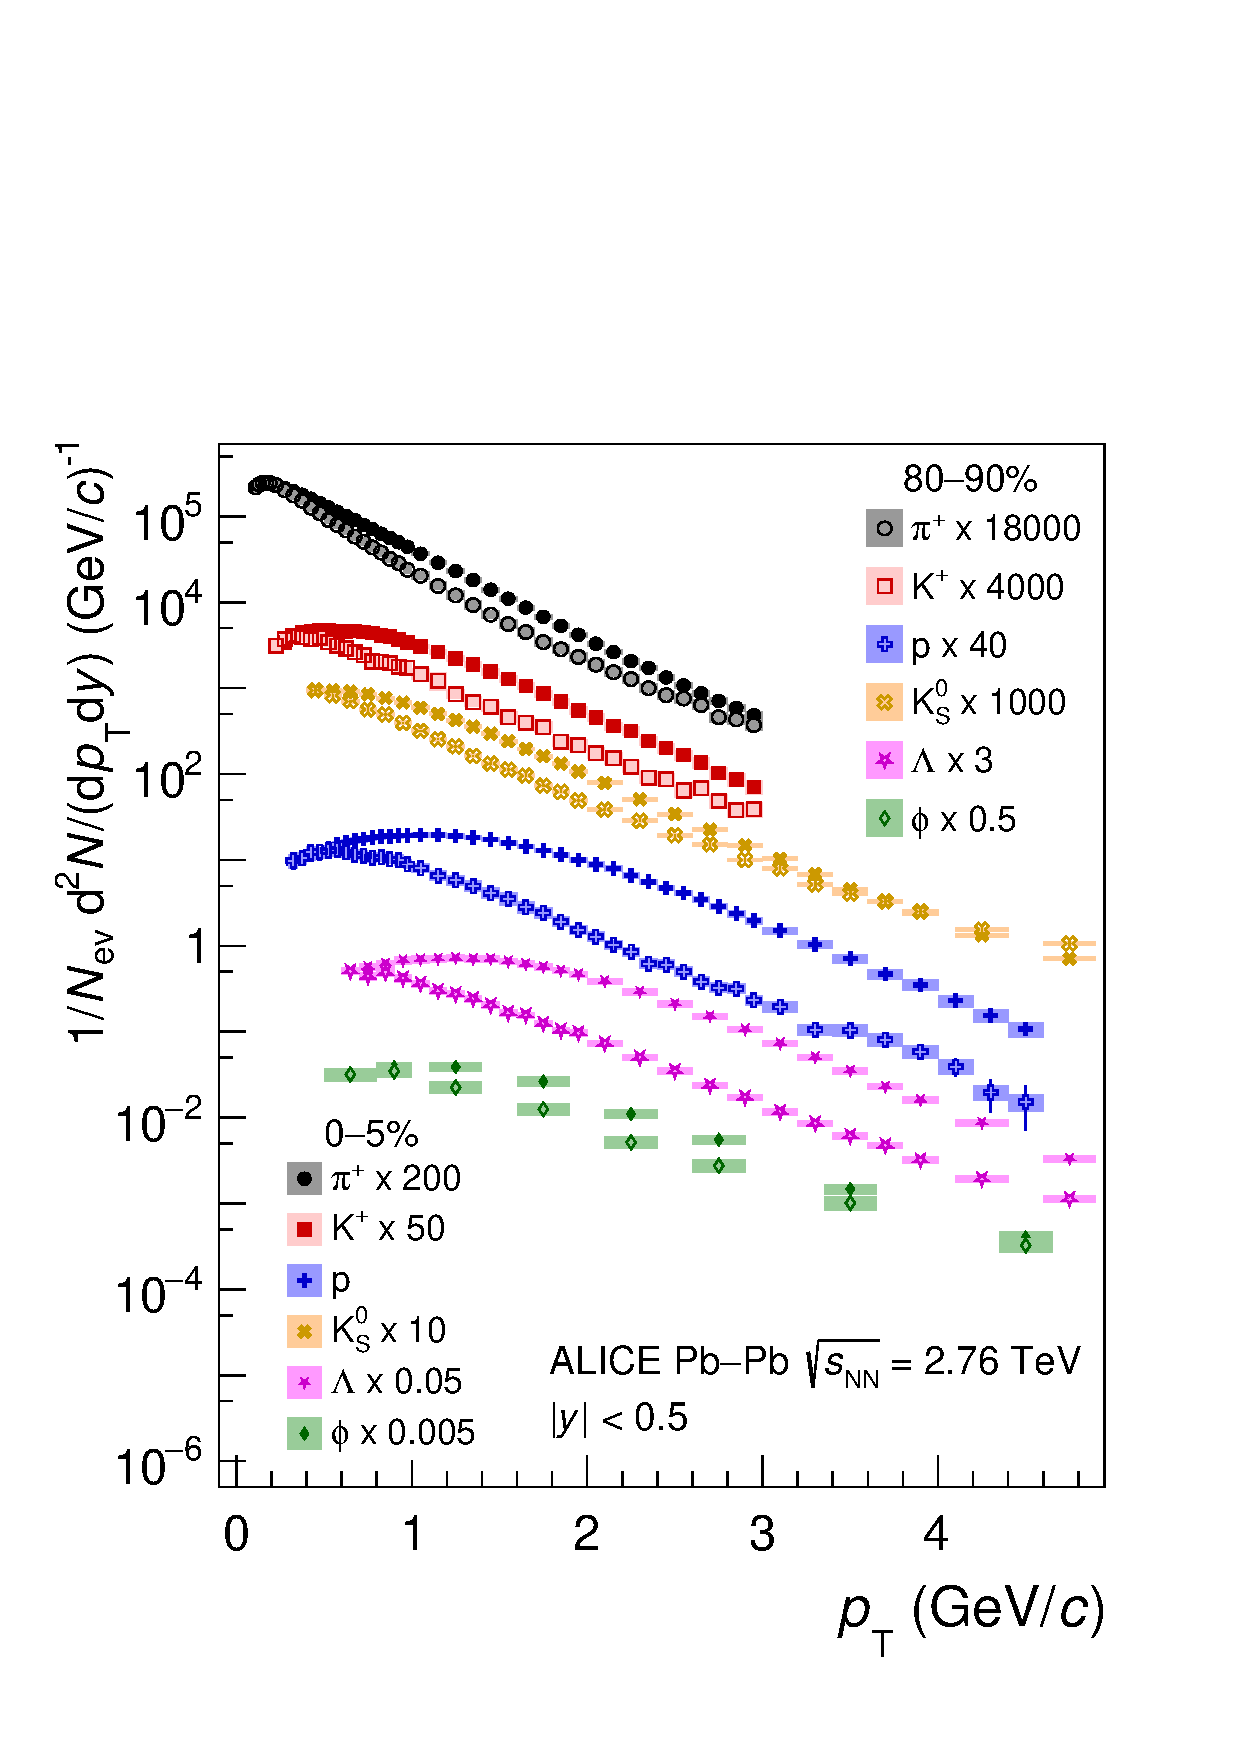
\includegraphics[width=.4\textwidth]{\imgpath/rfspectra.pdf}}}%\hspace{2em}
\subfloat[][]{\adjustbox{valign=m}{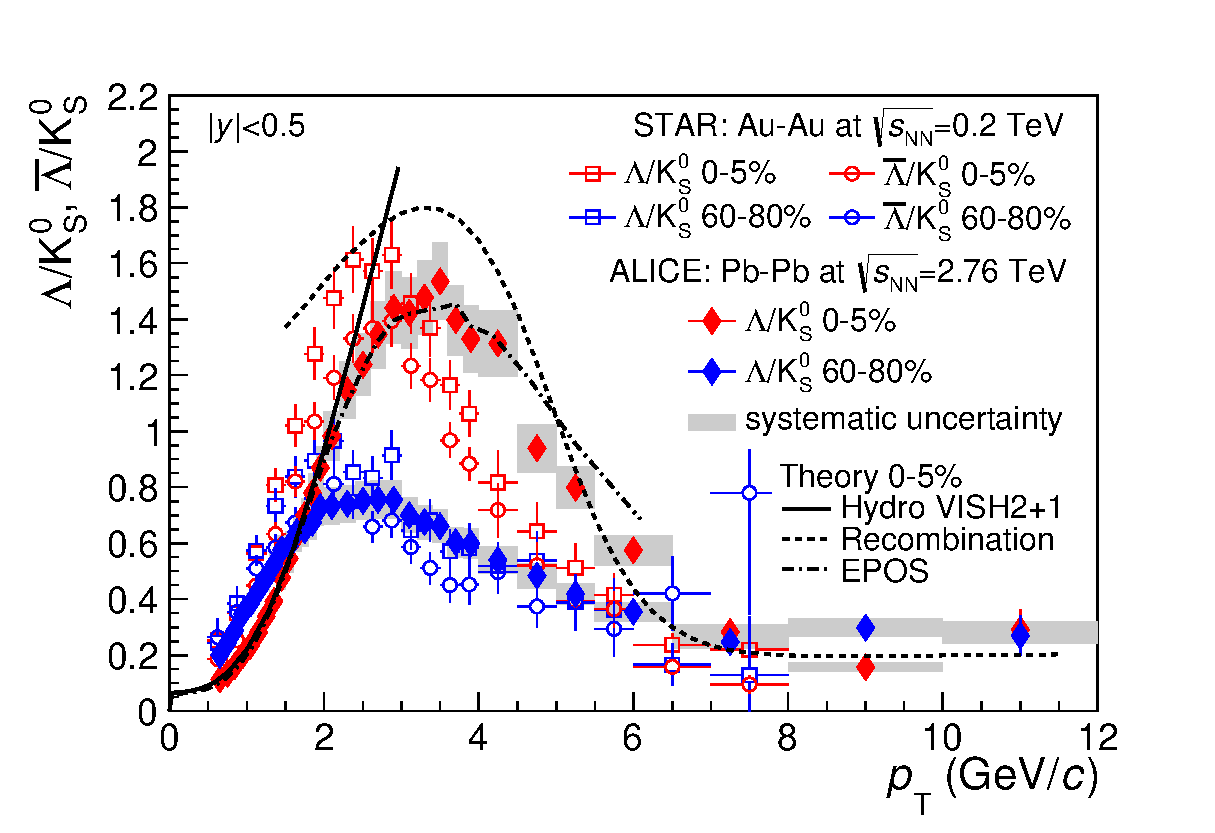
\includegraphics[width=.59\textwidth]{\imgpath/ltok.eps}}}
\caption{\textbf{(a)} Transverse momentum spectra of light-flavour hadrons in central $0-5\%$ and peripheral $80-90\%$ Pb-Pb collisions scaled by arbitrary factors to enhance the visibility. \cite{alicecollaborationALICEExperimentJourney2022, alicecollaborationCentralityDependenceRm2013, alicecollaborationRmSRm2013, alicecollaboration8920Phi2015} \textbf{(b)} \LA to \KOs ratios of transverse momentum spectra in Pb-Pb collisions at the LHC and Au-Au collisions at RHIC for central $0-5\%$ events (red) and peripheral $60-80\%$ events (blue). \cite{alicecollaborationRmSRm2013}}
\label{fig:colls:rflow}
\end{figure}

The flow coefficients can be experimentally extracted using various methods, including two-particle azimuthal correlations (as shown in Fig.~\ref{fig:colls:aflow}), and are typically studied as a function of event multiplicity. It is important to note that these azimuthal correlations between particles due to anisotropic flow are long-range, i.e.\ present consistently across the entire pseudorapidity range $\Delta \eta$ (the so-called ``ridge") \cite{luzumFlowFluctuationsLongrange2011}, which makes them distinguishable from similarly appearing ``non-flow" short-range correlations coming from jet fragmentation and resonance decays.
 
Moreover, measurements of $v_2$ in AA collisions for different particle species reveal a mass dependence in the low-\pt region, and a baryon/meson dependence in the intermediate \pt region, with baryons having approximately $1.5$ times higher values \cite{alicecollaborationEllipticFlowIdentified2015}. This suggests that the flow of hadrons is built up from its deconfined constituents.

\begin{figure}[H]
\subfloat[][]{\adjustbox{valign=m}{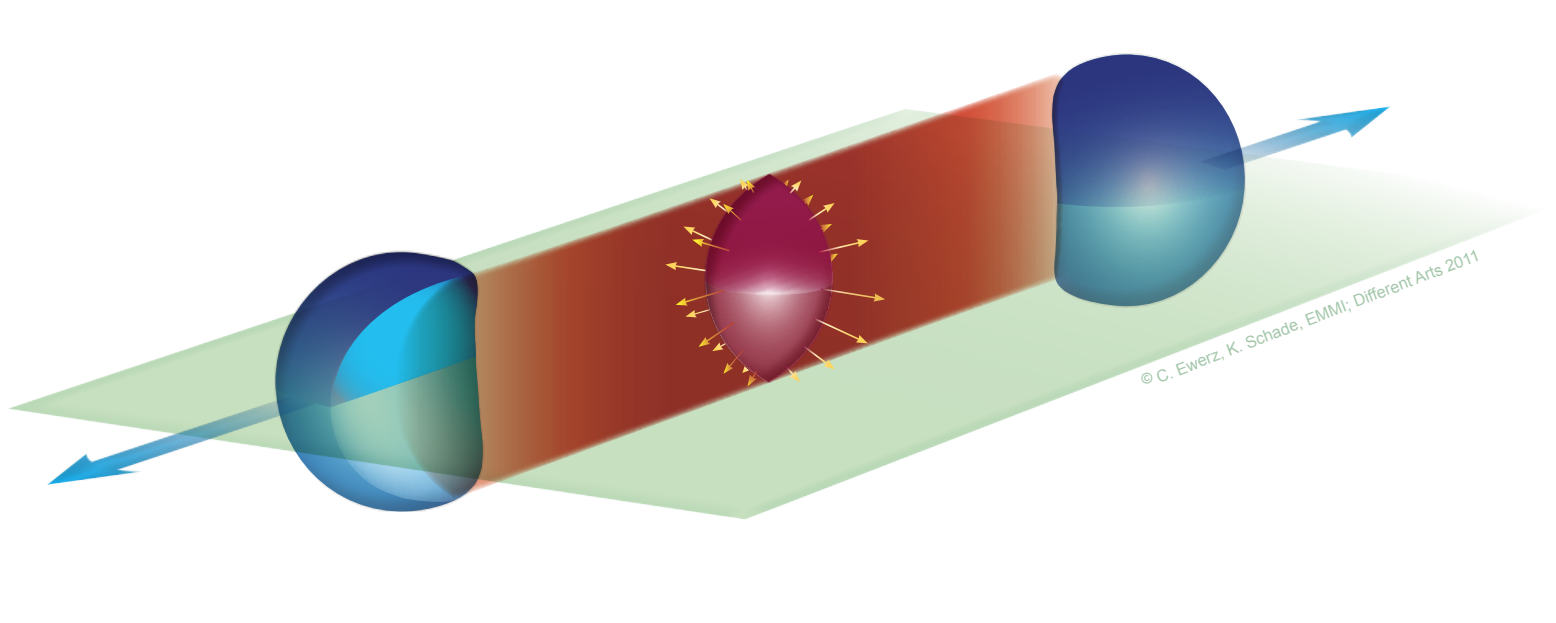
\includegraphics[width=.45\textwidth]{\imgpath/almond.png}}}\hspace{1em}
\subfloat[][]{\adjustbox{valign=m}{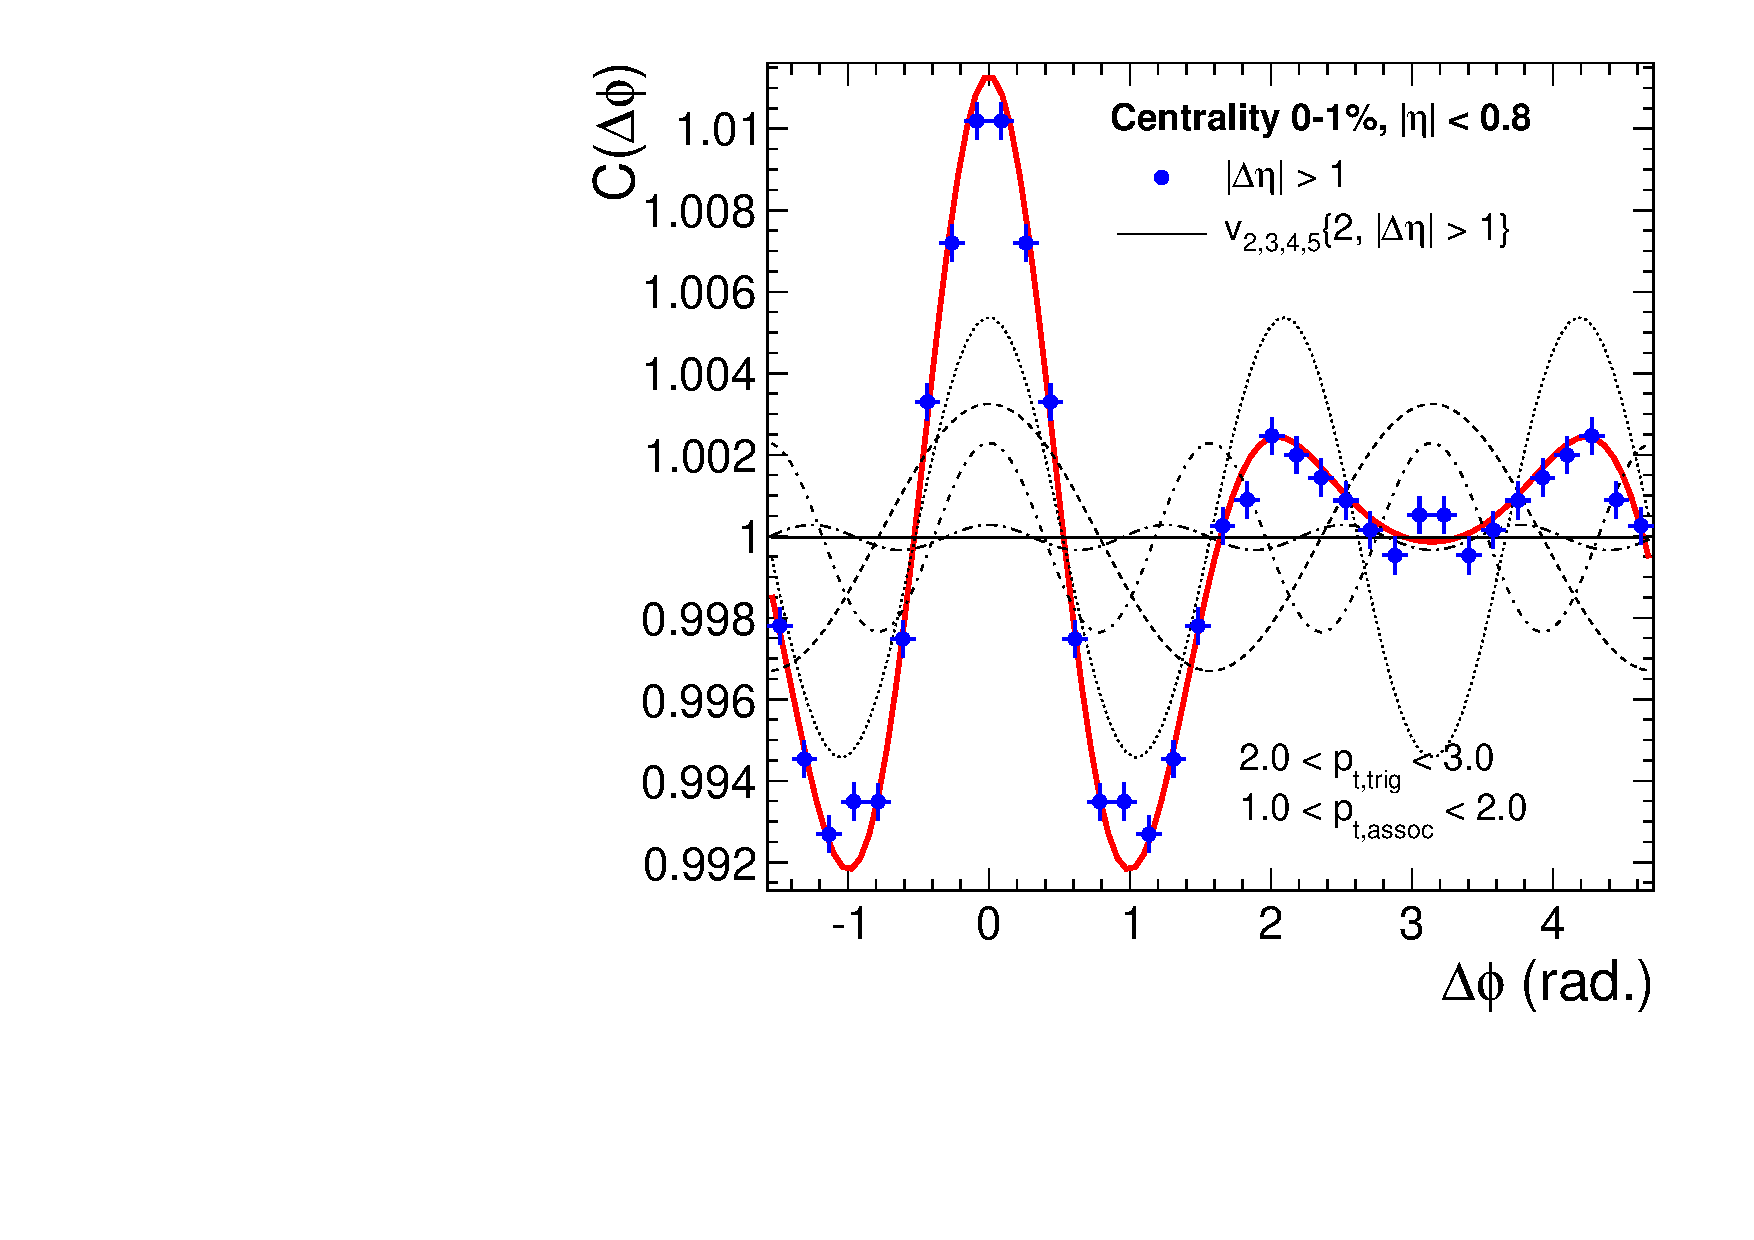
\includegraphics[width=.45\textwidth]{\imgpath/harmonics.pdf}}}
\caption{\textbf{(a)} Illustration of a collision of ultra-relativistic heavy nuclei and the overlapping region with pressure gradients (yellow). \cite{schadeApplicationsHolographyStrongly2012} \textbf{(b)} Correlation function of the relative azimuthal angle between a trigger particle and an associated particle, separated by a pseudorapidity gap, measured in central Pb-Pb collisions. The contributions from the elliptical, triangular, quadrupolar, and pentapolar harmonics are shown as different dashed lines. \cite{alicecollaborationHigherHarmonicAnisotropic2011}}
\label{fig:colls:aflow}
\end{figure}

\subsection{Jet quenching}

In AA collisions, partons produced in hard scattering processes interact with the colour charges in the quark-gluon plasma, resulting in the loss of energy through collisions and gluon bremstsstrahlung. This phenomenon is known as jet quenching and modifies or even "quenches" the parton shower \cite{gyulassyJetQuenchingDense1990, wangEffectJetQuenching1998}. In the factorisation theorem in Eq.~\ref{eq:intro:facto}, this corresponds to the medium-modification of the fragmentation functions. Studies of parton energy loss and jet quenching often use the transport coefficient $\hat{q}$, which describes the average \pt loss of a parton per a mean free path in the plasma and corresponds to the medium opacity

Jet quenching is one of the most important probes into the structure and dynamical properties of the QGP, since the hard partons experience its entire evolution, similarly to the case of heavy quarkonia discussed in Sec.~\ref{sec:colls:quarkonia}. It can also be compared with a large body of sound theoretical calculations \cite{gyulassyNonAbelianEnergyLoss2000} and MC simulations \cite{zappMonteCarloModel2009} based on QCD. Experimentally, jet quenching can manifest as suppression of the jet yield or even its complete disappearence, due to the energy loss of partons in the medium and their re-scattering. \cite{alicecollaborationALICEExperimentJourney2022}

Figure~\ref{fig:colls:jetquenching} displays such an AA event with a large jet imbalance and juxtaposes it with a pp event, where the leading and the recoil jet need to be balanced in azimuth due to conservation laws. Further effects and fields of study of jet quenching include the modification of jet substructures and shapes.

\begin{figure}[H]
\subfloat[][]{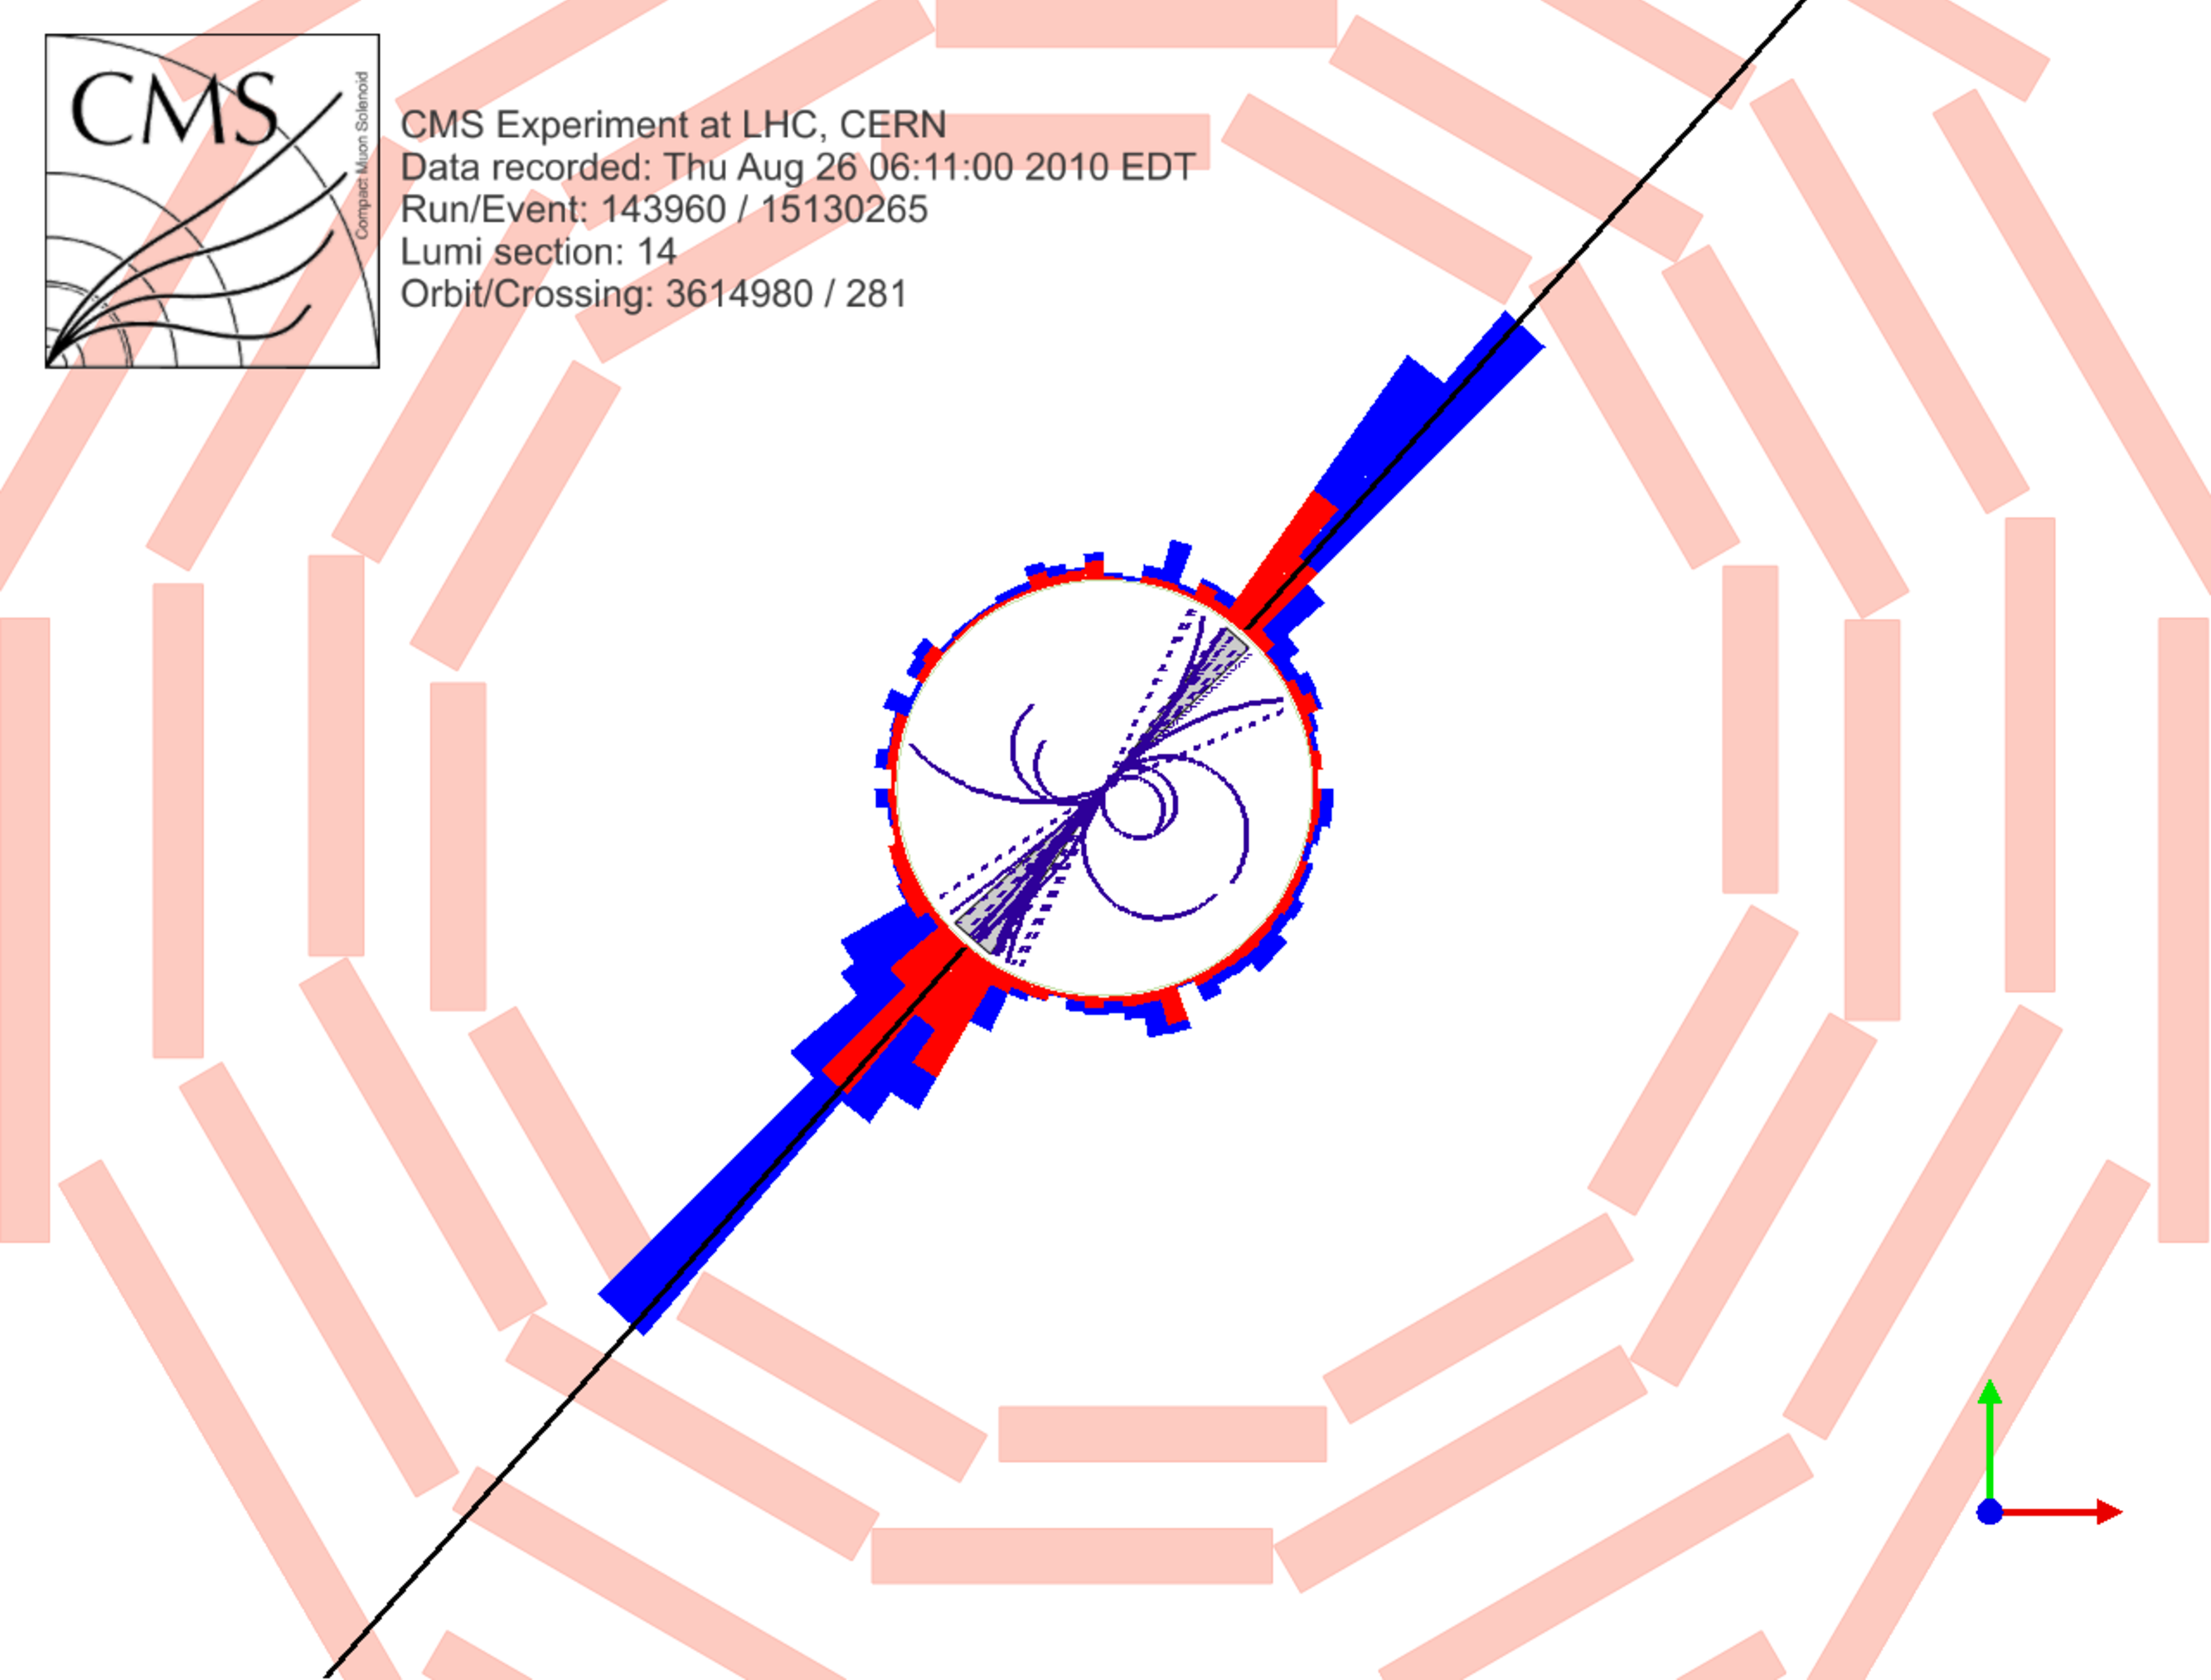
\includegraphics[height=11em]{\imgpath/DijetPP.pdf}}\hspace{2em} 
\subfloat[][]{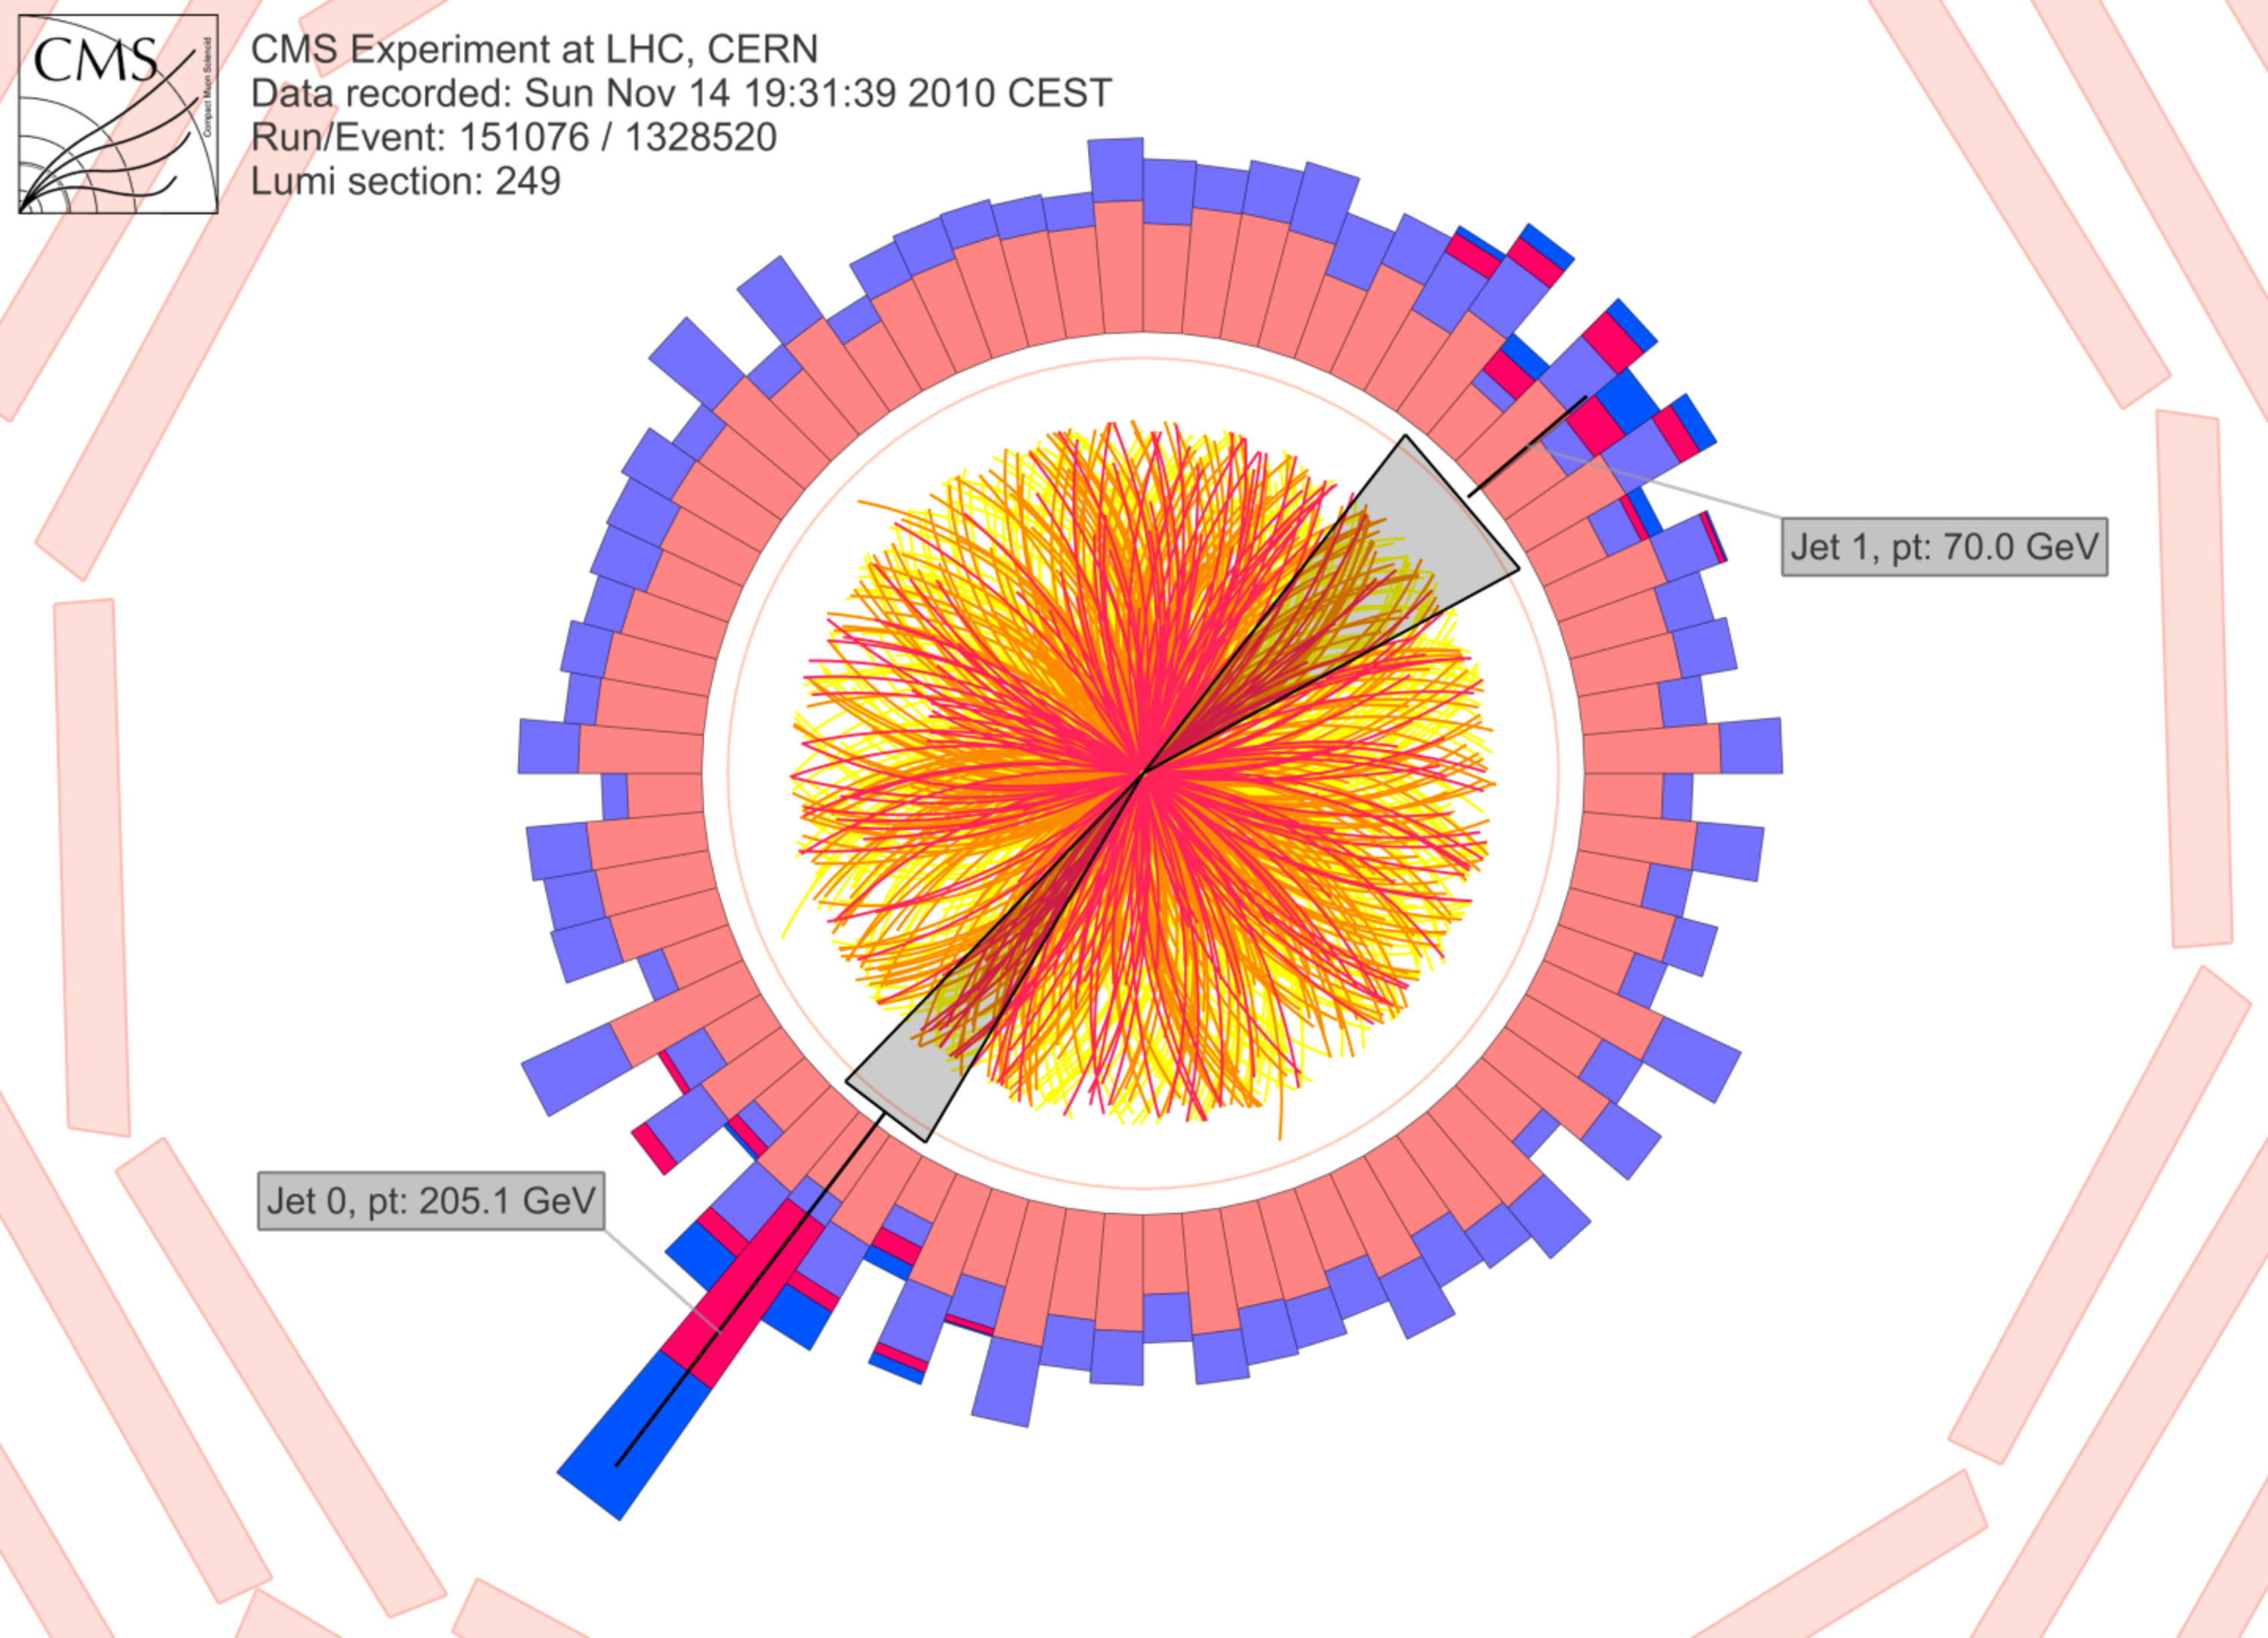
\includegraphics[height=11em]{\imgpath/DijetAA.pdf}}
\caption{Event displays from CMS in azimuthal plane showing a collision of \textbf{(a)} pp and \textbf{(b)} Pb-Pb with a dijet. The red and blue columns correspond to energy deposits in the detector calorimeters. \cite{cmsCMSCollisionEvents2010, niidaSignaturesQGPRHIC2021}}
\label{fig:colls:jetquenching}
\end{figure}

\subsection{Cold nuclear matter effects}

It should be noted that apart from the QGP, other effects come into play due to the fact that the collision involves two nuclei instead of two protons. These effects are important caveats to bear in mind and include:

\begin{enumerate}
\item Nuclear (anti-)shadowing: Reflects the modification in production due to differences in nPDFs and PDFs. \cite{vogtShadowingEffectsPsi2015}
\item Cronin effect: Describes the initial parton energy loss due to scatterings in the nuclear medium and broadens measured \pt spectra. \cite{croninProductionHadronsLarge1975}
\item Nuclear absorption: Describes the dissociation of particles due to their interactions with the passing-by nuclear remnants \cite{wongIntroductionHighenergyHeavyion1990}. It is generally negligible at LHC energies.
\item Co-mover absorption: This is the effect of inelastic interactions with the hadron gas. \cite{ferreiroExcitedCharmoniumSuppression2015}
\end{enumerate}

These effects can be isolated and quantified in pA or very peripheral AA collisions.

\section{QGP phenomena in small systems}\label{sec:colls:qgpss}

Measurements within the last decade have shown that certain QGP phenomena can also be observed in high-multiplicity events of pp collisions at LHC energies, which challenges the traditional assumption that QGP is only produced in AA collisions. This has sparked debates about the existence of QGP in pp collisions and, to a lesser degree, about the absence of QGP in AA collisions, despite the extensive experimental evidence.

Furthermore, the observed behavior of these phenomena indicates that the role of event multiplicity \Nch may be more significant than the collision system size. This has led to ongoing efforts to establish a consistent and seamless link between the paradigms of pp and AA collisions.

\subsubsection*{Strangeness and charm enhancement}

ALICE measurements on $\LA/\pi$, $\XI/\pi$, and $\Omega/\pi$ ratios demonstrate that the production rates of particles containing strange quarks increase faster with multiplicity than those containing only u and d quarks \cite{adamEnhancedProductionMultistrange2017}. This also depends on the strangeness content -- the effect is the strongest for $\Omega$ and vanishes for protons. Furthermore, the evolution to larger systems seems to be continuous with respect to \Nch. The measurements can be seen in Fig.~\ref{fig:colls:ssstrangeness} \cite{alicecollaborationALICEExperimentJourney2022}.

To contrast the strangeness measurements with charm, the $J/\psi \ /\pi$ ratio also shows a clear increase in yield with increasing \Nch in pp collisions, as is shown in Fig.~\ref{fig:colls:ssstrangeness} \cite{alicecollaborationMultiplicityDependencePsi2020, alicecollaborationObservationMultiplicityDependence2022}. However, this comes with an important caveat: high-multiplicity events are biased to have enhanced hard processes, as discussed further in Chapter~\ref{chap:rt}. Moreover, the evolution of this phenomenon is also not continuous with \Nch when going from pp collisions at \sppt{13} to \snnt{5.02}, which can also be explained by the fact that charm quarks are produced solely in hard scattering processes, the rates of which depend on the collision system and center-of-mass energy.

\begin{figure}[H]
\subfloat[][]{\adjincludegraphics[trim={0 0 {.48\width} 0},clip,height=15em]{\imgpath/ss_strangeness1.pdf}}\hspace{2em}
\subfloat[][]{\adjincludegraphics[trim={0 0 {.948\width} 0},clip,height=15em]{\imgpath/ss_strangeness2.pdf}\adjincludegraphics[trim={{.52\width} 0 0 0},clip,height=15em]{\imgpath/ss_strangeness2.pdf}} 
\caption{Ratios of integrated yields of \textbf{(a)} various light-flavour hadrons \cite{adamEnhancedProductionMultistrange2017} and \textbf{(b)} charm mesons \cite{alicecollaborationMultiplicityDependencePsi2020, alicecollaborationObservationMultiplicityDependence2022} to pions as a function of multiplicity in pp, p-Pb, and Pb-Pb collisions. \cite{alicecollaborationALICEExperimentJourney2022}}
\label{fig:colls:ssstrangeness}
\end{figure}

\subsubsection*{Anisotropic flow}

Azimuthal correlations and anisotropic flow measurements in small collision systems exhibit features similar to those observed in AA collisions, hinting at the presence of collective expansion \cite{cmscollaborationEvidenceCollectivityPp2017}. However, in small systems, these measurements are particularly challenging due to their large sensitivity to non-flow effects, such as jet fragmentation or resonance decays, which can mimic the features of collective flow. 

While models using hydrodynamic-like descriptions seem to be able to describe $v_2$ results (despite the fact that their assumption $\lambda \ll L$ is not valid) \cite{wellerOneFluidRule2017}, especially at high multiplicities, the interpretation of the results in small systems is still under investigation. The values of elliptic flow $v_2$ seem to be comparable to those in low-multiplicity Pb-Pb collisions, although the evolution of $v_2$ across different system sizes does not appear to be smooth. The measurements from CMS displaying a clear ridge in high-multiplicity events \cite{cmscollaborationEvidenceCollectivityPp2017} and the $v_2$ results from ALICE \cite{alicecollaborationInvestigationsAnisotropicFlow2019} can be seen in Fig.~\ref{fig:colls:ssv2}.

\begin{figure}[H]
\subfloat[][]{\adjincludegraphics[trim={0 {0.67\height} 0 0},clip,width=0.45\textwidth]{\imgpath/ss_ridge1.pdf}}
\subfloat[][]{\adjincludegraphics[trim={0 {0.67\height} 0 0},clip,width=0.45\textwidth]{\imgpath/ss_ridge2.pdf}}\\
\adjincludegraphics[trim={0 {0.7\height} 0 0},clip,width=0.8\textwidth]{\imgpath/ss_v2.pdf}
\subfloat[][]{\adjincludegraphics[trim={0 0 0 {0.966\height}},clip,width=0.8\textwidth]{\imgpath/ss_v2.pdf}}
\caption{\textbf{(a, b)} Two-dimensional two-particle correlation functions of charged hadrons in low (left) and high (right) multiplicity events of pp collisions at \sppt{13}. \cite{cmscollaborationEvidenceCollectivityPp2017} \textbf{(c)} Elliptic flow measured using two-particle cumulants with a pseudorapidity separation in pp, p-Pb, Xe-Xe, and Pb-Pb collisions as a function of multiplicity. \cite{alicecollaborationInvestigationsAnisotropicFlow2019}}
\label{fig:colls:ssv2}
\end{figure}

\subsubsection*{Radial flow}

Measurements of the ratio of \LA to \KOs \pt spectra ratio were also studied in pp collisions with differing \Nch, see Fig.~\ref{fig:colls:ssrflow} \cite{alicecollaborationMultiplicityDependenceMulti2020}. The boost of a collectively expanding system, as expected in the context of radial flow, should have a greater impact on heavier hadrons, leading to an enhancement of the baryon-to-meson ratio at intermediate \pt. This enhancement is observed in the \LA/\KOs ratio, its magnitude increases with increasing \Nch and the peak position shifts towards higher values collisions, consistent with the hydrodynamic picture. The increase at intermediate momenta leads to a corresponding depletion at low \pt. High-\pt (as well as integrated) \LA/\KOs ratios exhibit essentially no (or minor) multiplicity dependence. This observation also applies to proton-to-pion ratios. 

Recent studies have also investigated the charmed baryon-to-meson ratio $\LA_c/\mathrm{D^0}$, with similar findings, although measurements with smaller uncertainties are still required. Fig.~\ref{fig:colls:ssrflow} presents the corresponding results.

\begin{figure}[H]
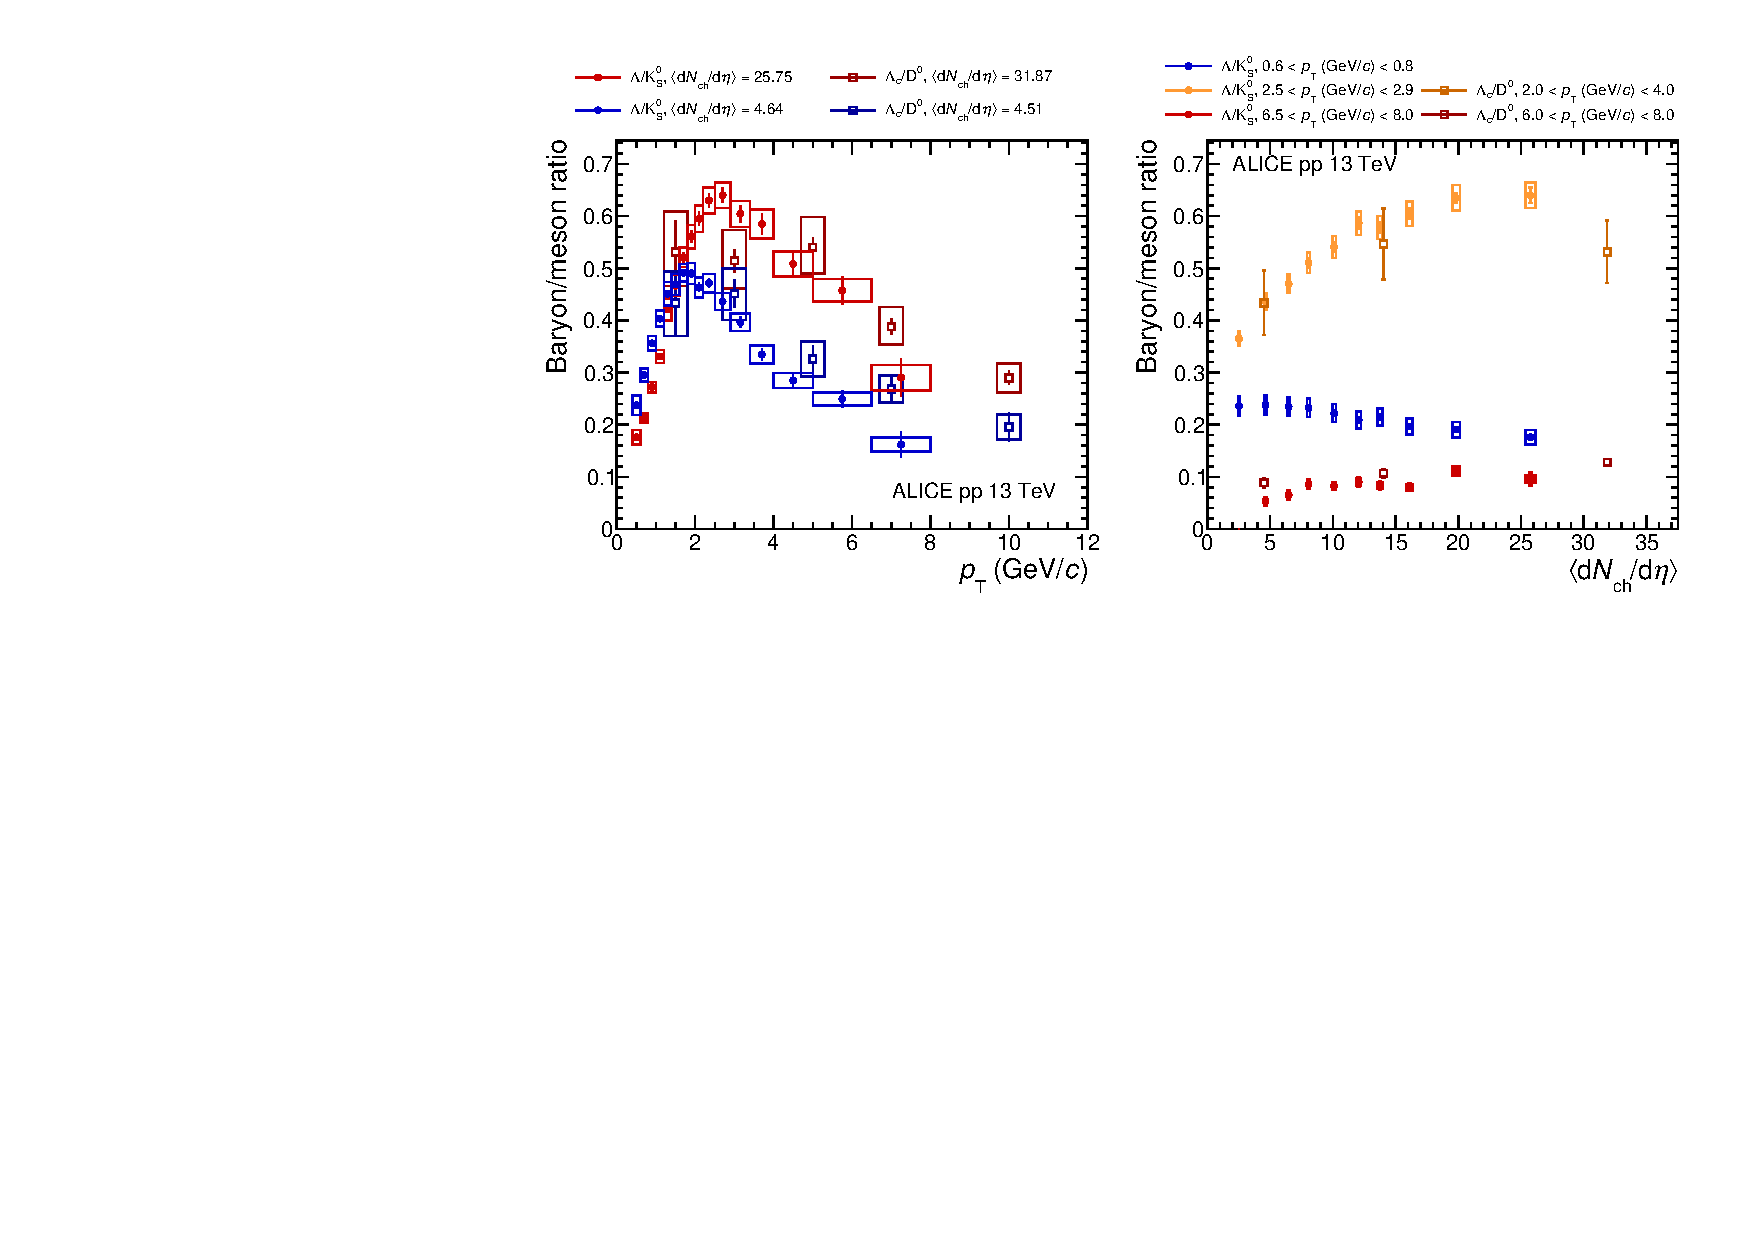
\includegraphics[width=.90\textwidth]{\imgpath/ss_rflow.pdf}
\caption{Baryon-to-meson ratios shown as the \pt differentials (left) and integrated yields in various \pt ranges as a function of multiplicity (right) for the \LA/\KOs and $\LA_c$/$\mathrm{D^0}$ in pp collisions at \sppt{13}. \cite{alicecollaborationMultiplicityDependenceMulti2020, alicecollaborationObservationMultiplicityDependence2022, alicecollaborationALICEExperimentJourney2022}}
\label{fig:colls:ssrflow}
\end{figure}

\subsubsection*{Sequential suppression of $\Upsilon$ states}

While defining $R_\mathrm{AA}$ to compare high-multiplicity and low-multiplicity events is unclear, and measuring yields as a function of \Nch is complicated by its biases related to the hardness of primary scatterings, it is worthwhile to investigate the ratio of excited-to-ground states of quarkonia as a function of \Nch.

Interestingly, these results \cite{cmscollaborationInvestigationEventactivityDependence2020} exhibit a decrease with increasing \Nch, resembling the pattern of sequential suppression due to QGP deconfinement. Even more remarkable, this dependence disappears in low-sphericity, jet-dominated, events (event shape observables such as sphericity are discussed in more detail in Chapter~\ref{chap:sphero}). These findings, reported in Fig.~\ref{fig:colls:ssupsilon}, suggest that the dependence on \Nch is solely influenced by the UE, rather than jets. As event multiplicity grows larger, excited $\Upsilon$ states become relatively less likely to be measured compared to the ground state.

These results indicate the need for a better understanding of $\Upsilon$ hadronization and the role UE may play in it. They also raise the question of whether the ground state is enhanced rather than the excited states being suppressed. Additionally, the effects of the mass differences must also be considered. However, the fact that low-sphericity, jet-dominated events have the same ratios as high-sphericity, UE-dominated events at low \Nch argues against these ideas.

An important caveat to note is that hadronic decays (which are dominant) of the heavy $\Upsilon$ states may result in tens of produced particles \cite{behrendsInclusiveHadronProduction1985}. Therefore, even minor discrimination against the excited states could hypothetically be correlated with a substantial but trivial increase in the accompanying \Nch. To the author's knowledge, there are currently no available phenomenological descriptions of the observed behavior, which further limits potentially groundbreaking interpretations.

\begin{figure}[H]
\subfloat[][]{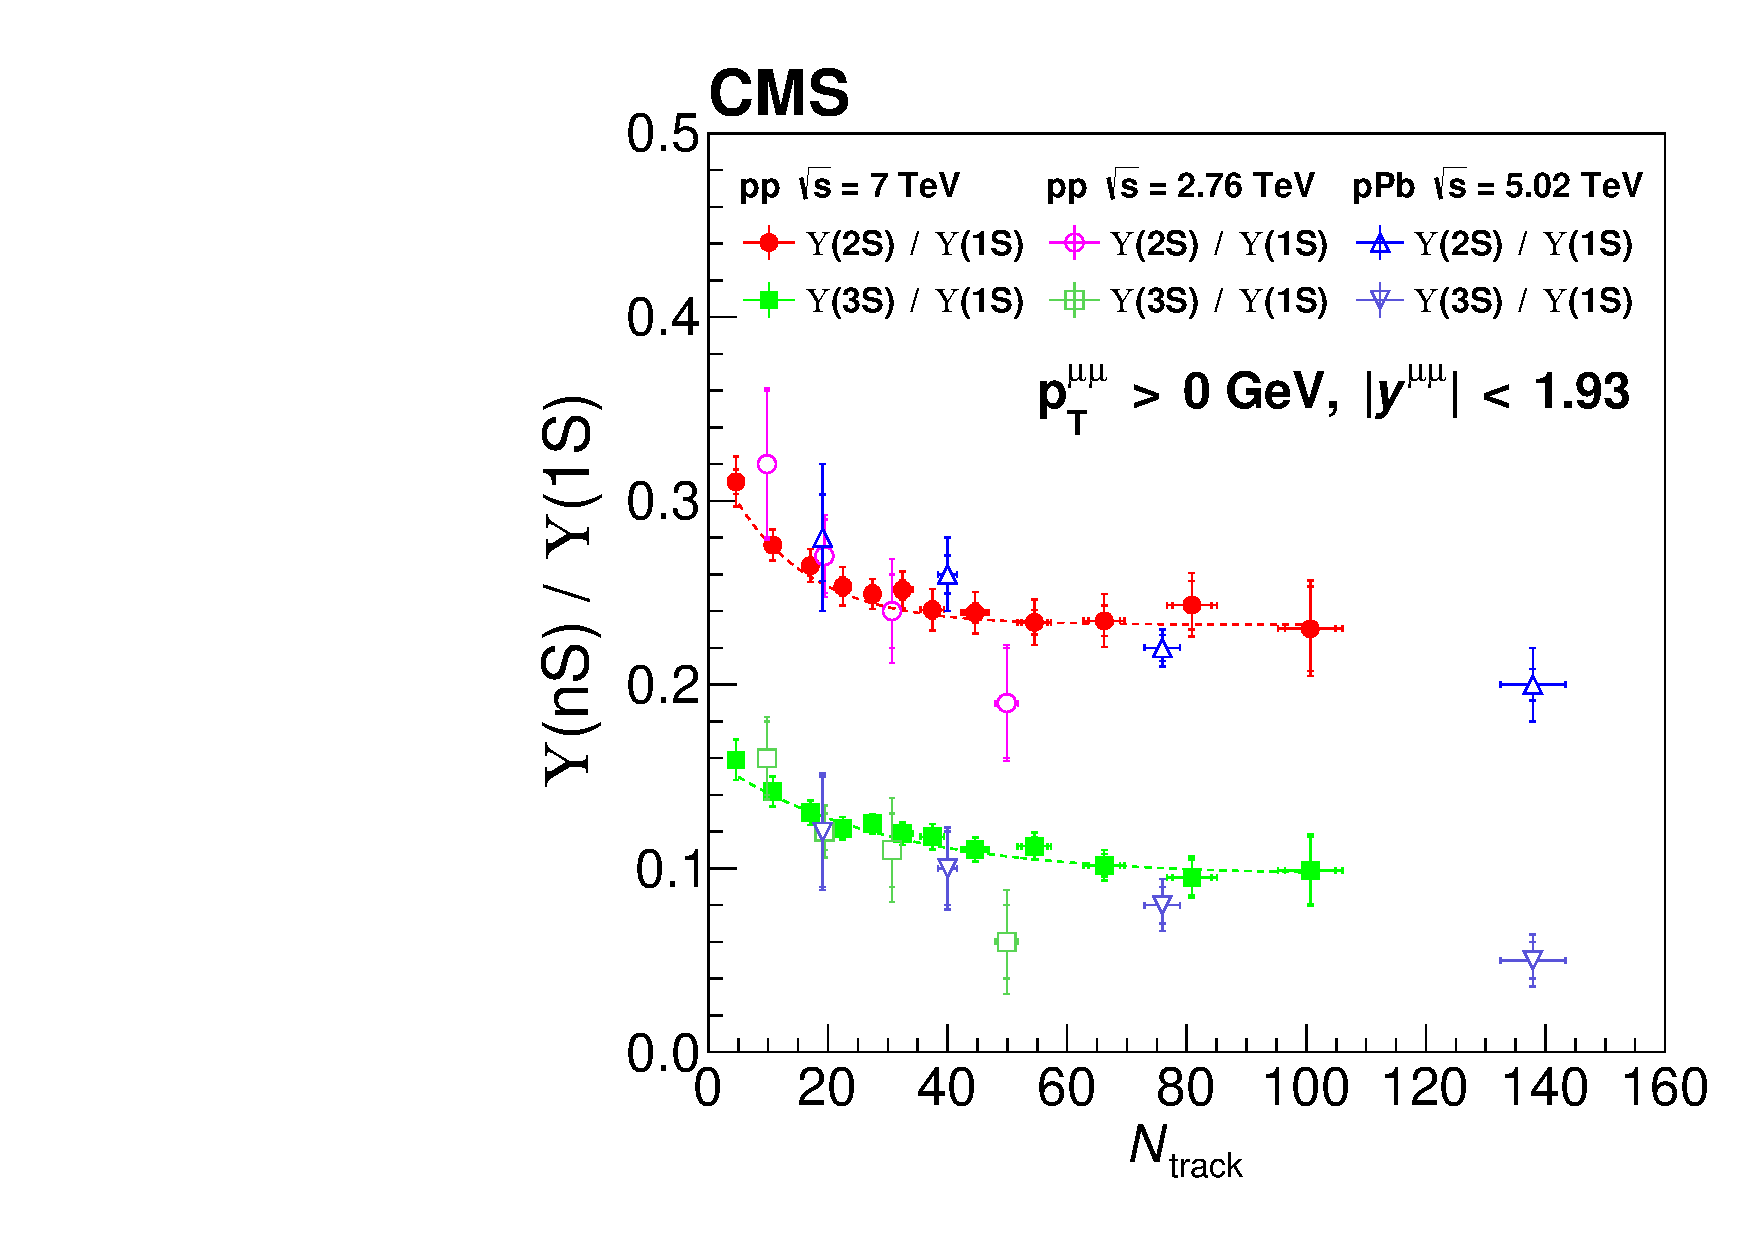
\includegraphics[width=.40\textwidth]{\imgpath/ss_ups1.pdf}}\hspace{1em} 
\subfloat[][]{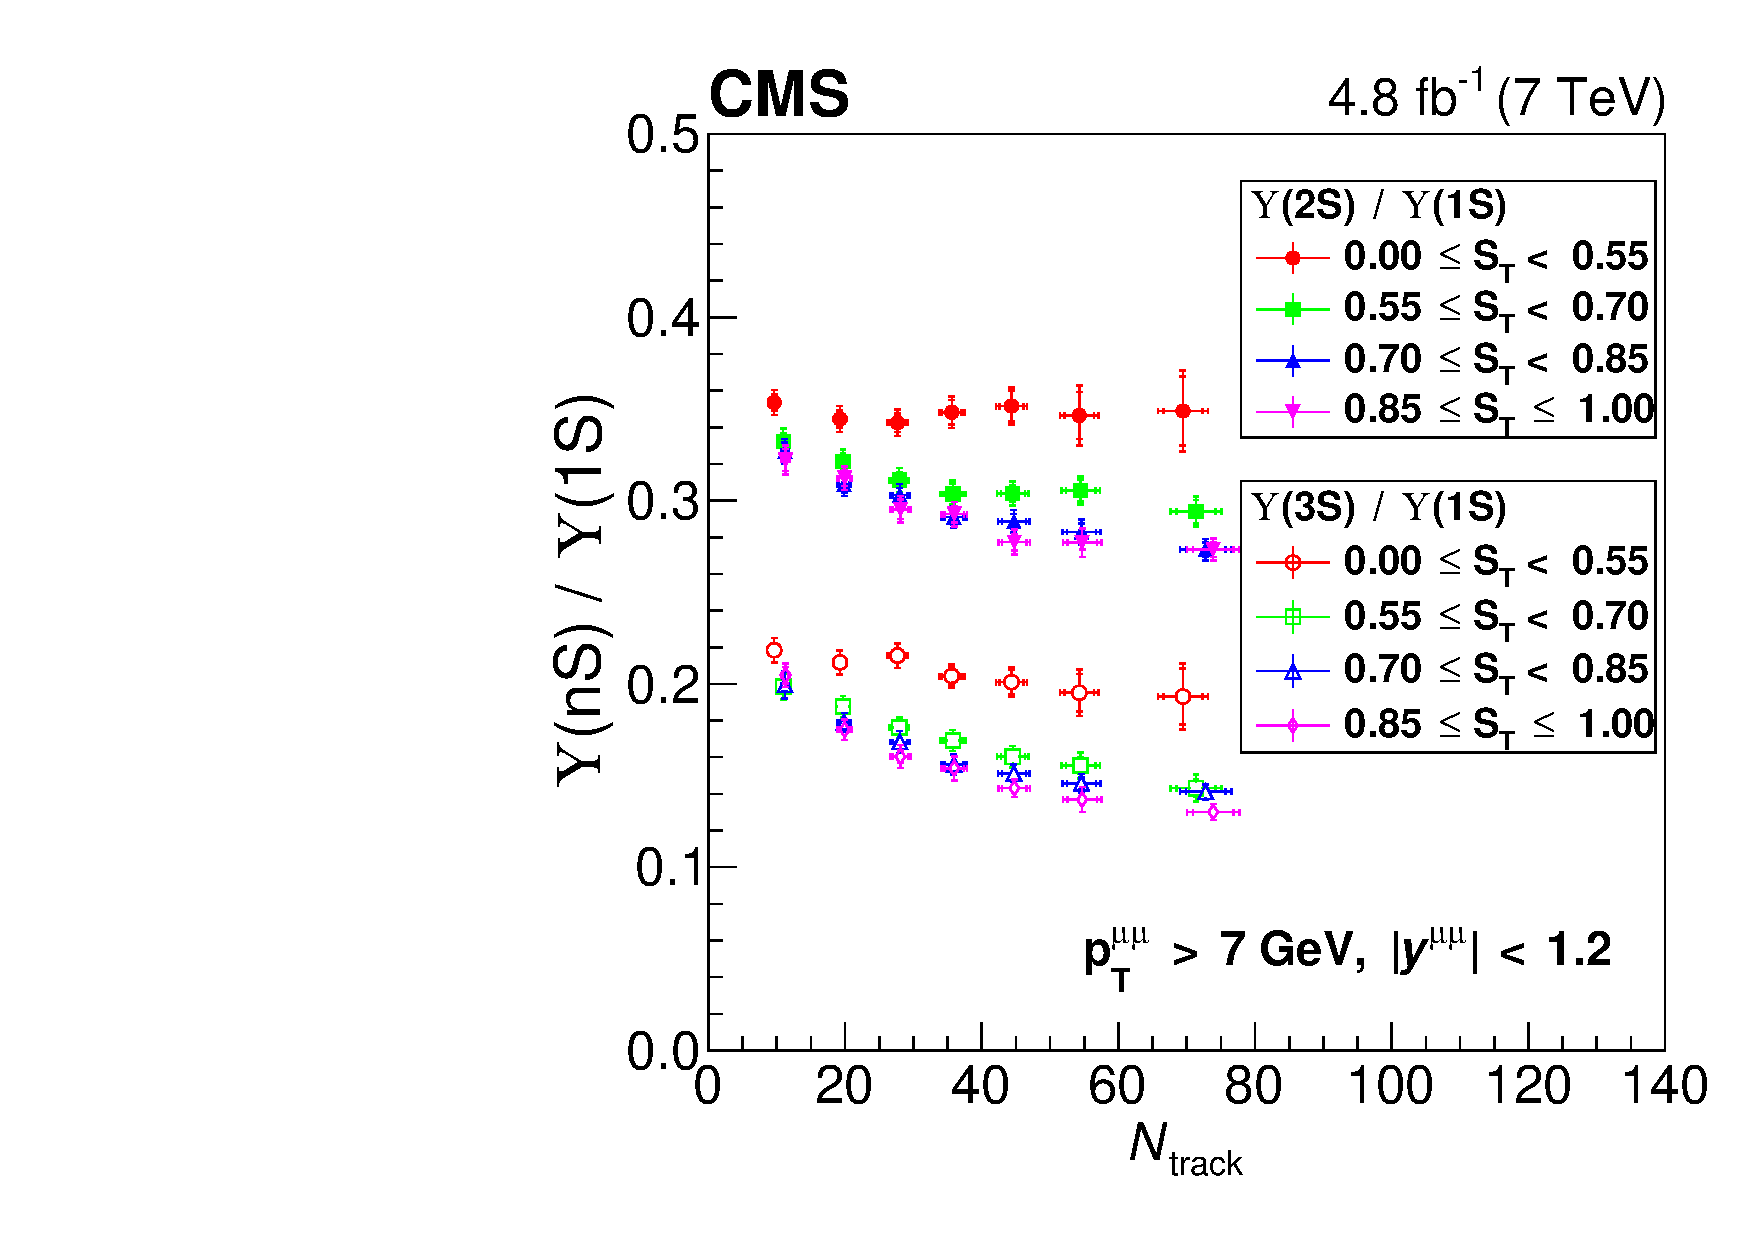
\includegraphics[width=.40\textwidth]{\imgpath/ss_ups2.pdf}}
\caption{The $\Upsilon$(2S)/$\Upsilon$(1S) and $\Upsilon$(3S)/$\Upsilon$(1S) ratios of measured yields in pp collisions as a function of \textbf{(a)} multiplicity, compared with p-Pb results, and \textbf{(b)} multiplicity and transverse sphericity, with the di-muon transverse momentum $\pt^{\mu\mu}>\gevc{7}$. \cite{cmscollaborationInvestigationEventactivityDependence2020}}
\label{fig:colls:ssupsilon}
\end{figure}

\subsubsection*{Other QGP signatures}

If a QGP is formed in small systems with sufficient volumes, the effect of jet quenching should be observed. One can also expect to observe it, due to the fact that in small systems, high-\pt hadrons have been measured to have finite flow $v_2$ \cite{cmscollaborationEllipticFlowCharm2018}, which could indicate that hard partons interact with an expanding medium. Whilst theoretical approaches do not provide unambiguous answers on whether this phenomenon can be observed \cite{zakharovPartonEnergyLoss2014} or not \cite{chenCentralityDependenceProductions2015}, experimental results on jet quenching in both pp and p-Pb collisions are consistent with no observable effect, within uncertainties \cite{alicecollaborationConstraintsJetQuenching2018}. These results are mostly based on measuring jet yields as a function of event activity, although such measurements are challenging due to fluctuations and interplays between jet characteristics and event activity.

\subsection{Role of multiplicity}

The observations made above highlight the significance of studying the role of multiplicity \Nch. In contrast to AA collisions, high-multiplicity events in pp collisions do not arise from a mere increase in the amount of colliding matter, as the values of \Npart and \Ncoll are fixed:
\begin{align}
\Npart = 2 \, ,\quad \ \Ncoll = 1 \, .
\end{align} 

Additionally, due to the relatively constant initial system volume, high-\Nch pp events may exhibit energy densities that exceed the threshold for QGP formation, given that the highest \Nch values are similar to those observed in peripheral AA collisions, where QGP formation is observed.

Clearly, the picture is more complex and despite its simplicity as an event activity classifier, \Nch poses challenges when it comes to relating data to theory since it cannot be directly linked to the initial state, and multiplicities in different events may originate from entirely different processes.

To address these issues and gain a better understanding of the evolution between low and high multiplicities and the potential for QGP formation, this dissertation focuses on transverse spherocity \SOPT and underlying event activity \RT measurements. The goal of these studies is to provide a deeper insight into the relevant degrees of freedom involved.

%One expects a trivial difference as the pT spectra are being measured at midrapidity in the same kinematic region where the midrapidity multiplicity selection is done. However, the slope of the pT spectra at high-pT indicates that the midrapidity estimator selects harder and harder subnucleonic interactions as the multiplicity increases. The ratios obtained with the forward estimator do not show a change in slope at high-pT. Still, the hard high-pT production is more enhanced than soft low-pT production in highmultiplicity collisions and vice versa in low-multiplicity collisions. This implies that the scaling with multiplicity of soft and hard processes is fundamentally different in pp compared to nucleus–nucleus collisions.

%a study with PYTHIA 8 (Monash 2013 tune) shows that the forward multiplicity estimator has the strongest correlation between the number of MPIs and the multiplicity. For this reason, the forward multiplicity slicing is used for multiplicity selection in the rest of this section unless specifically noted otherwise. As the multiplicity selection is done on charged particles, a second advantage of the forward selection is that it does not create an imbalance between charged and neutral particles at midrapidity

\section{Phenomenological models}

The next parts of this thesis give an overview to phenomenological models and event generators pertinent to the measurements in Chapters~\ref{chap:sphero} and \ref{chap:rt}. Other generators, such as Herwig 7 \cite{bellmHerwigReleaseNote2020} or Sherpa \cite{bothmannEventGenerationSherpa2019}, are not discussed here.

\subsection{Pythia}

Pythia is a Monte Carlo event generator used to simulate full events of high-energy particle collisions, based mostly on approximately perturbative QCD, with some important non-perturbative aspects. With more than four decades of development, only a brief overview is given in this thesis, whilst detailed description can be found in Ref.~\cite{bierlichComprehensiveGuidePhysics2022, sjostrandPYTHIAEventGenerator2020}. It has a modular structure to simulate different aspects of the collision process and includes the simulation of the initial kinematics, hard scattering, multiple parton interactions, parton showering, and hadronization, which were all discussed in Chapter~\ref{chap:intro}. The various components of the event simulation, such as the matrix element for the primary scattering, or even the parton evolution, can also be replaced with external alternatives. 

Its current and in ALICE most widely used version is Pythia 8, specifically its Monash tune \cite{skandsTuningPYTHIAMonash2014}, incorporating colour reconnections. Pythia has also included the implementation of Angantyr \cite{bierlichAngantyrModelHeavyIon2018}, a new model for the simulation of collisions of nuclei.

A pp collision event, as simulated by Pythia, can be seen in the illustration in Fig.~\ref{fig:colls:pythia} and crudely structured as:
\begin{enumerate}
\item Relevant parton kinematics are determined based on the PDFs of the beam particles and nature of the event is decided (e.g.\ $Z^0$ production). Produced resonances decay.
\item All subsequent partonic activity is simulated. This includes the initial- and final-state parton radiation, MPIs, and handling of the beam particle remnants. Eventually, after the full parton shower evolutions, a full partonic structure and string configuration is given.
\item Hadronisation occurs by the Lund string model fragmentation. This part is completely non-perturbative and fully phenomenological. Unstable particles decay and a full final-state particle collection is obtained. \cite{sjostrandBriefIntroductionPYTHIA2008}
\end{enumerate}

\begin{figure}[H]
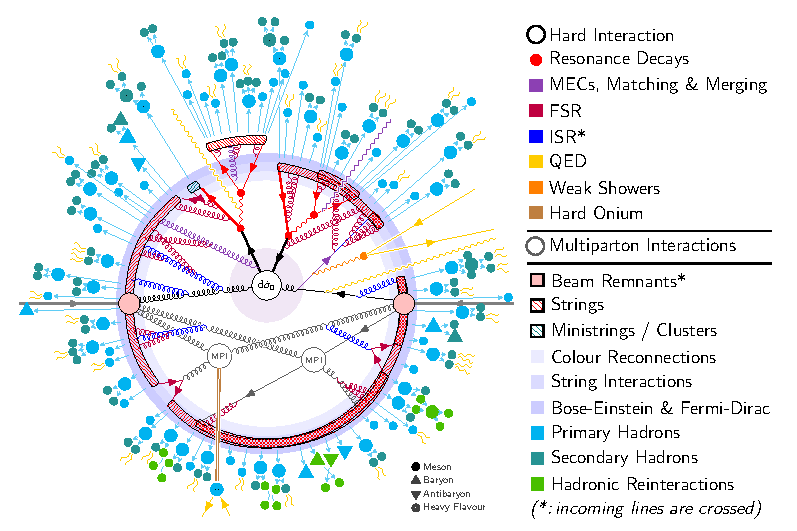
\includegraphics[width=.90\textwidth]{\imgpath/pythia.pdf}
\caption{Diagram depicting a full simulation of pp collision event with its various components. For full description, see Ref.~\cite{bierlichComprehensiveGuidePhysics2022}.}
\label{fig:colls:pythia}
\end{figure}

\subsection{String interactions and Ropes}

While some effects typically associated with QGP formation, such as radial flow, can be somewhat mimicked in Pythia by colour reconnection \cite{bierlichEffectsColourReconnection2015, ortizColorReconnectionFlowlike2013}, as touched upon in Sec.~\ref{sec:intro:cr}, it is not sufficient to describe the strangeness enhancement patterns observed in small systems.

Ideas that overlapping QCD strings in high-density environments interact and form higher-tension ropes date back to modelling AA collisions in 1984 \cite{biroColourRopeModel1984} and have been explored further \cite{sorgeColourRopeFormation1992}, specifically in the framework of the DIPSY model \cite{bierlichEffectsOverlappingStrings2015}. This ``rope hadronisation" approach is also incorporated similarly in Pythia 8 and can be included in its simulations, which in the context of this dissertation will be referred to as the Pythia 8 Ropes tune.

In Pythia, strings are considered overlapping on purely geometrical considerations and utilise a parameter $\alpha$ to quantify the size of strings relatively to the proton radius. Combining two strings follows an algebra based on the SU($3$) group, described below, following a more detailed discussion in Ref.~\cite{bierlichEffectsOverlappingStrings2015}.

A $q\bar{q}$ string can be viewed as a SU($3$) triplet $\mathbf{3}$. Stacking another string suggests adding another triplet and forming a multiplet with quantum numbers $p$, corresponding to the number of coherent triplets $\mathbf{3}$ (e.g.\ all red), and $q$, corresponding to the number of coherent antitriplets $\mathbf{\bar{3}}$ (e.g.\ all anti-blue). Using a $\{p,q\}$ notation, the algebra for multiplets is as follows:
\begin{align}
\{1,0\} \otimes \{1,0\} = \{2,0\} \oplus \{0,1\} \quad ,\\
\{1,0\} \otimes \{0,1\} = \{1,1\} \oplus \{0,0\} \quad .
\end{align}

The first equation, physically, corresponds to merging of two colour strings with colour flows going in the same direction (same $q\bar{q}$ orientation), merging into a rope. When the colours are the same (e.g.\ both red), the result is a sextet rope $\mathbf{6}$, $\{2,0\}$. In other cases (e.g.\ red and blue), the result is an anti-triplet rope $\mathbf{\bar{3}}$, $\{0,1\}$ (corresponding to anti-green---green string). This algebra is illustrated in Fig.~\ref{fig:colls:ropes}.

The second equation describes stacking a triplet $\mathbf{3}$ with an anti-triplet $\mathbf{\bar{3}}$ (opposite colour flows and $q\bar{q}$ orientation). This results either in a gluon octet $\mathbf{8}$, $\{1,1\}$, or a singlet $\mathbf{1}$, $\{0,0\}$, with destructive interference and no colour flow.

The tension of the produced rope $\tilde{\kappa}$ is proportional to the quadratic Casimir operator $C_2$. When normalising to the tension of a single string $\kappa$, e.g.\ a $\{1,0\}$ triplet, the relative increase is given by
\begin{align}\label{eq:colls:string}
\frac{\tilde{\kappa}}{\kappa} = \frac{C_2( \{p,q\})}{C_2 ( \{1,0\})} = \frac{p^2+q^2+pq+3p+3q}{4} \quad ,
\end{align}
so in the example of adding two red triplets, the resulting $\{2,0\}$ rope tension is $\tilde{\kappa}=5/2$.

During hadronisation, the rope is assumed to break not entirely at once, but rather one string at a time. For the purpose of considering the probability of creating new quarks in (\ref{eq:intro:tunnel}), the effective tension from the $\{p,q\}\to \{p-1,q\}$ transition is given by (\ref{eq:colls:string}) and corresponds to
\begin{align}
\tilde{\kappa}_\mathrm{eff} = \frac{2p+q+2}{4}\kappa \quad.
\end{align}

This means that in the example of the $\{2,0\}$ rope breaking, the first quark creation comes with relative effective tension $\tilde{\kappa}_\mathrm{eff} = 3\kappa/2$, and the second one with the normal value of $\tilde{\kappa}_\mathrm{eff}=\kappa$.

The strangeness production suppression factor in (\ref{eq:intro:rho}) then becomes modified as
\begin{align}
\tilde{\rho} = \rho^{\frac{\kappa}{\tilde{\kappa}_\mathrm{eff}}} \quad ,
\end{align}
which makes it evident that overlapping many strings ($\tilde{\kappa}_\mathrm{eff} \to \infty$) results in $\tilde{\rho} \to 1$ and strange quarks are produced at the same rate as up and down. 

Furthermore, ideas for further interactions between strings, such as ``string shoving", wherein overlapping strings may repel each other due to transverse pressure from their excess energy, have also been developed. Such mechanisms produce effects similar to a hydrodynamically expanding medium, e.g.\ long-range anisotropic flow. \cite{bierlichShovingModelCollectivity2016}

\begin{figure}[H]
\subfloat[][]{\adjustbox{valign=m}{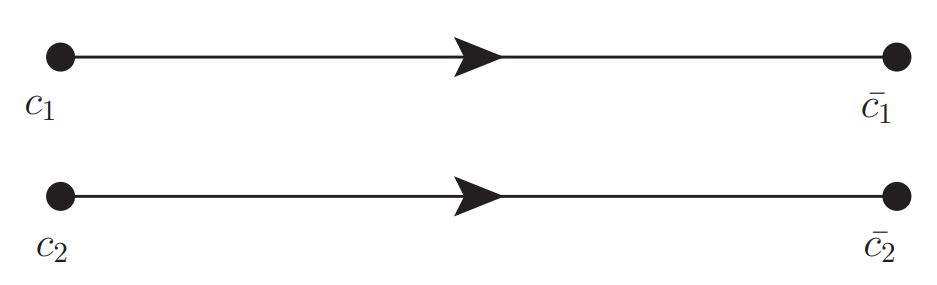
\includegraphics[width=.3\textwidth]{\imgpath/ropes1.png}}}\hspace{1em}
\subfloat[][]{\adjustbox{valign=m}{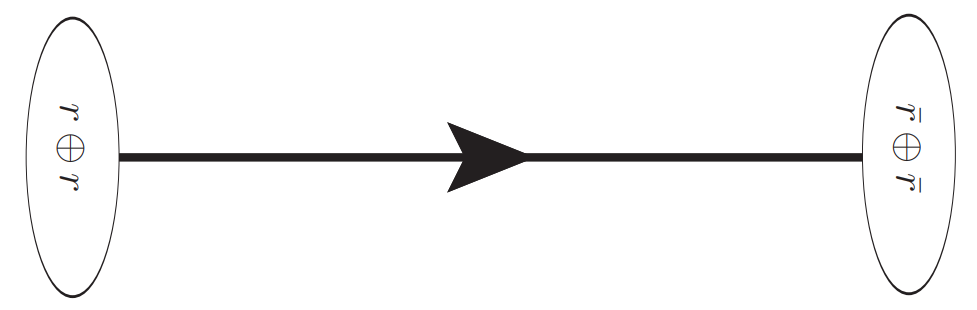
\includegraphics[width=.3\textwidth]{\imgpath/ropes2.png}}}\hspace{1em}
\subfloat[][]{\adjustbox{valign=m}{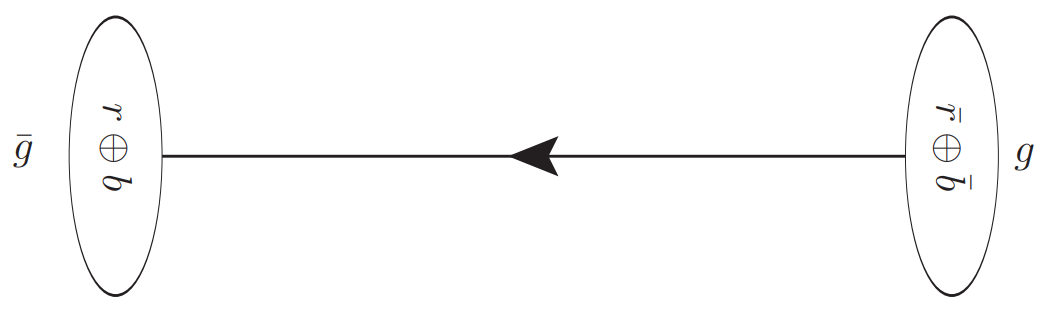
\includegraphics[width=.3\textwidth]{\imgpath/ropes3.png}}}
\caption{\textbf{(a)} Illustration of stacking two colour flow strings, triplets with colours $c_1$ and $c_2$.  \textbf{(b)} Rope sextet resulting from adding two coherent triplets, $c_1 = c_2$, $\{2,0\}$. \textbf{(c)} Resulting rope anti-triplet coming from adding two incoherent triplets, $c_1 \neq c2$, $\{0,1\}$. Illustrations are by C.\ Bierlich.}
\label{fig:colls:ropes}
\end{figure}


\subsection{EPOS LHC}

EPOS is an event generator built on the Gribov-Regge theory \cite{drescherPartonBasedGribovReggeTheory2001}, wherein several partons undergo multiple scatterings, each consisting of the hard scattering component as well as initial and final state linear parton emission. Together, they form a so-called parton ladder and correspond to a ``cut" pomeron exchange \cite{wernerPartonLadderSplitting2006}. The parton ladder represents a (mostly) longitudinally flowing colour field, a ``flux tube", which may hadronise via pair production.

To model the full collision process, EPOS combines a two-component core-corona approach. When the density of flux tubes in a given volume exceeds a parameter $\rho_0$, the core is formed. Conversely, flux tubes escaping the volume (usually with higher \pt) make up the corona. The core is assumed to evolve hydrodynamically, corresponding to a QGP droplet, and then hadronises collectively, where smaller core segments form hadrons following a statistical ensemble. Since the relative amount of core- and corona-related particle production can vary continuously, EPOS models can be used to describe pp, pA, and AA collisions using a single paradigm. \cite{pierogEPOSLHCTest2015}

EPOS models have been successful particularly at modelling soft-QCD physics and, apart from collider physics, are also widely used in studies of cosmic rays \cite{pierogEPOSModelUltra2009}. Throughout this dissertation, an adaptation of EPOS called EPOS LHC \cite{pierogEPOSLHCTest2015} is mostly used and shown, which only parametrises the flow dynamics of the core instead of implementing a full hydrodynamic simulation. Diagrams illustrating the partonic structure and core-corona mixing can be seen in Fig.~\ref{fig:colls:epos}.

\begin{figure}[H]
\subfloat[][]{\adjustbox{valign=m}{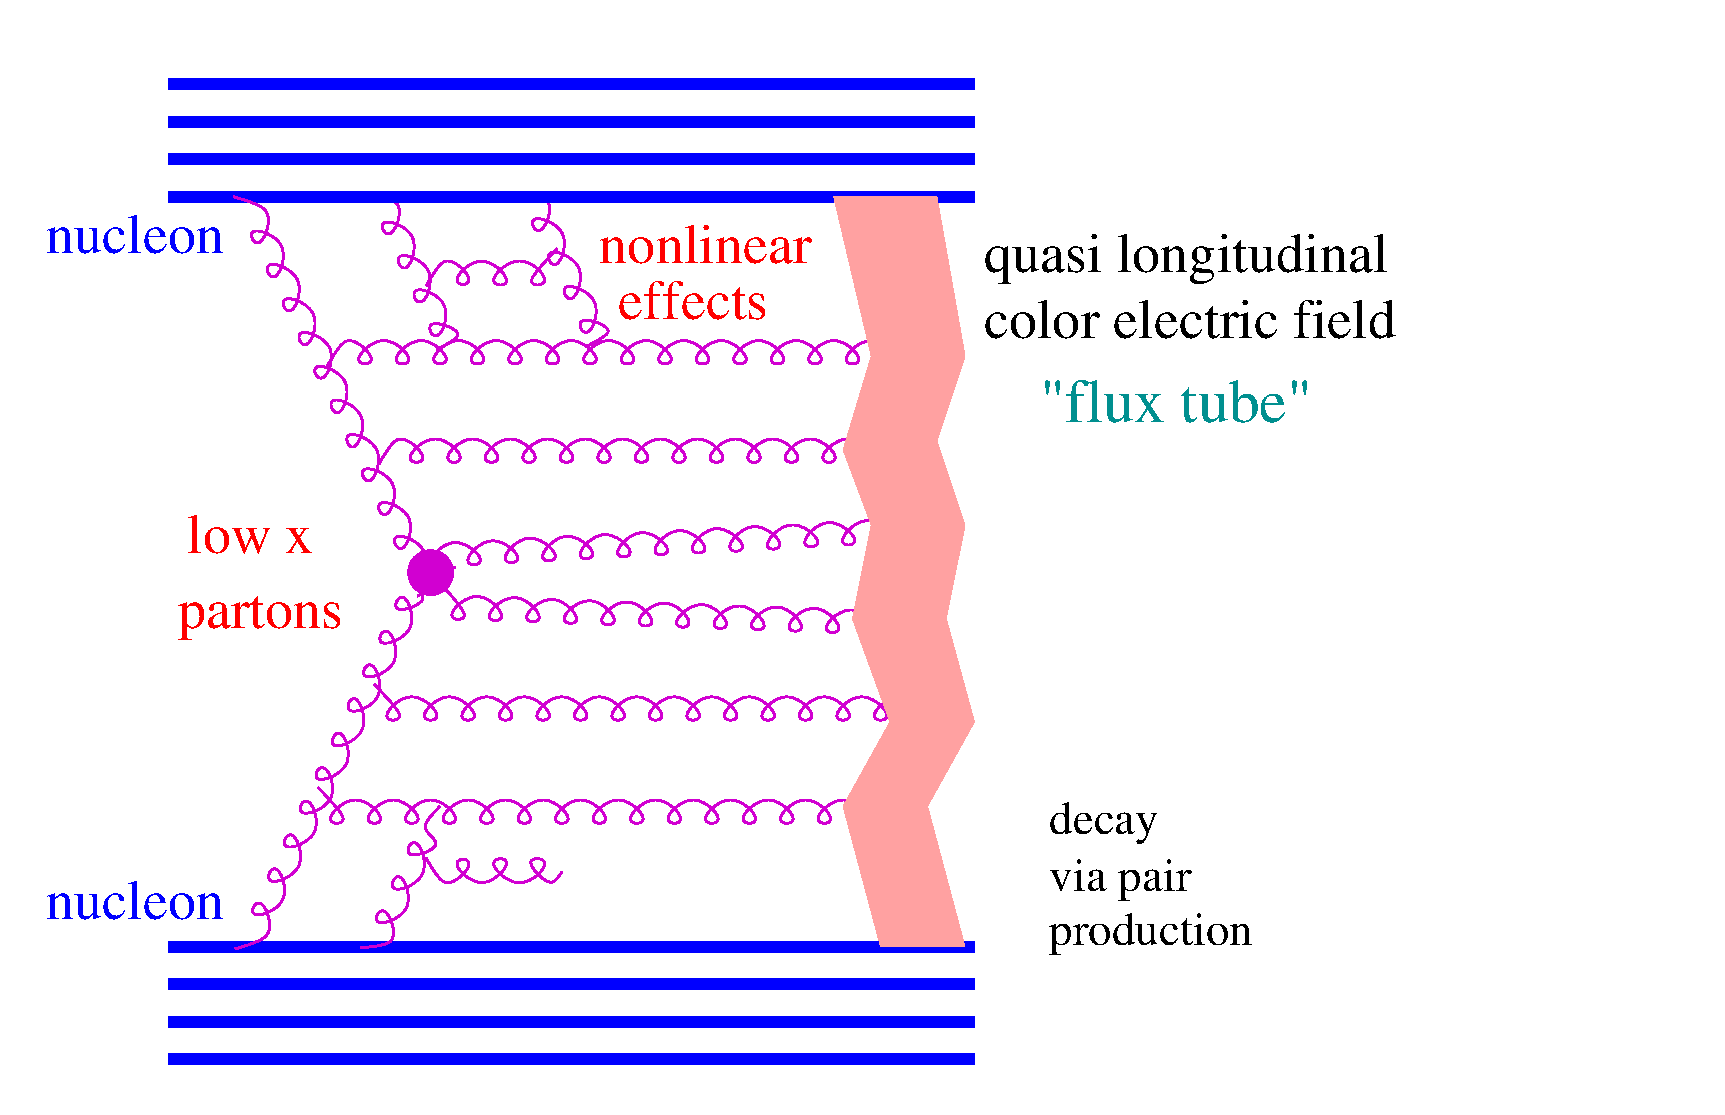
\includegraphics[width=.49\textwidth]{\imgpath/flux.eps}}}
\subfloat[][]{\adjustbox{valign=m}{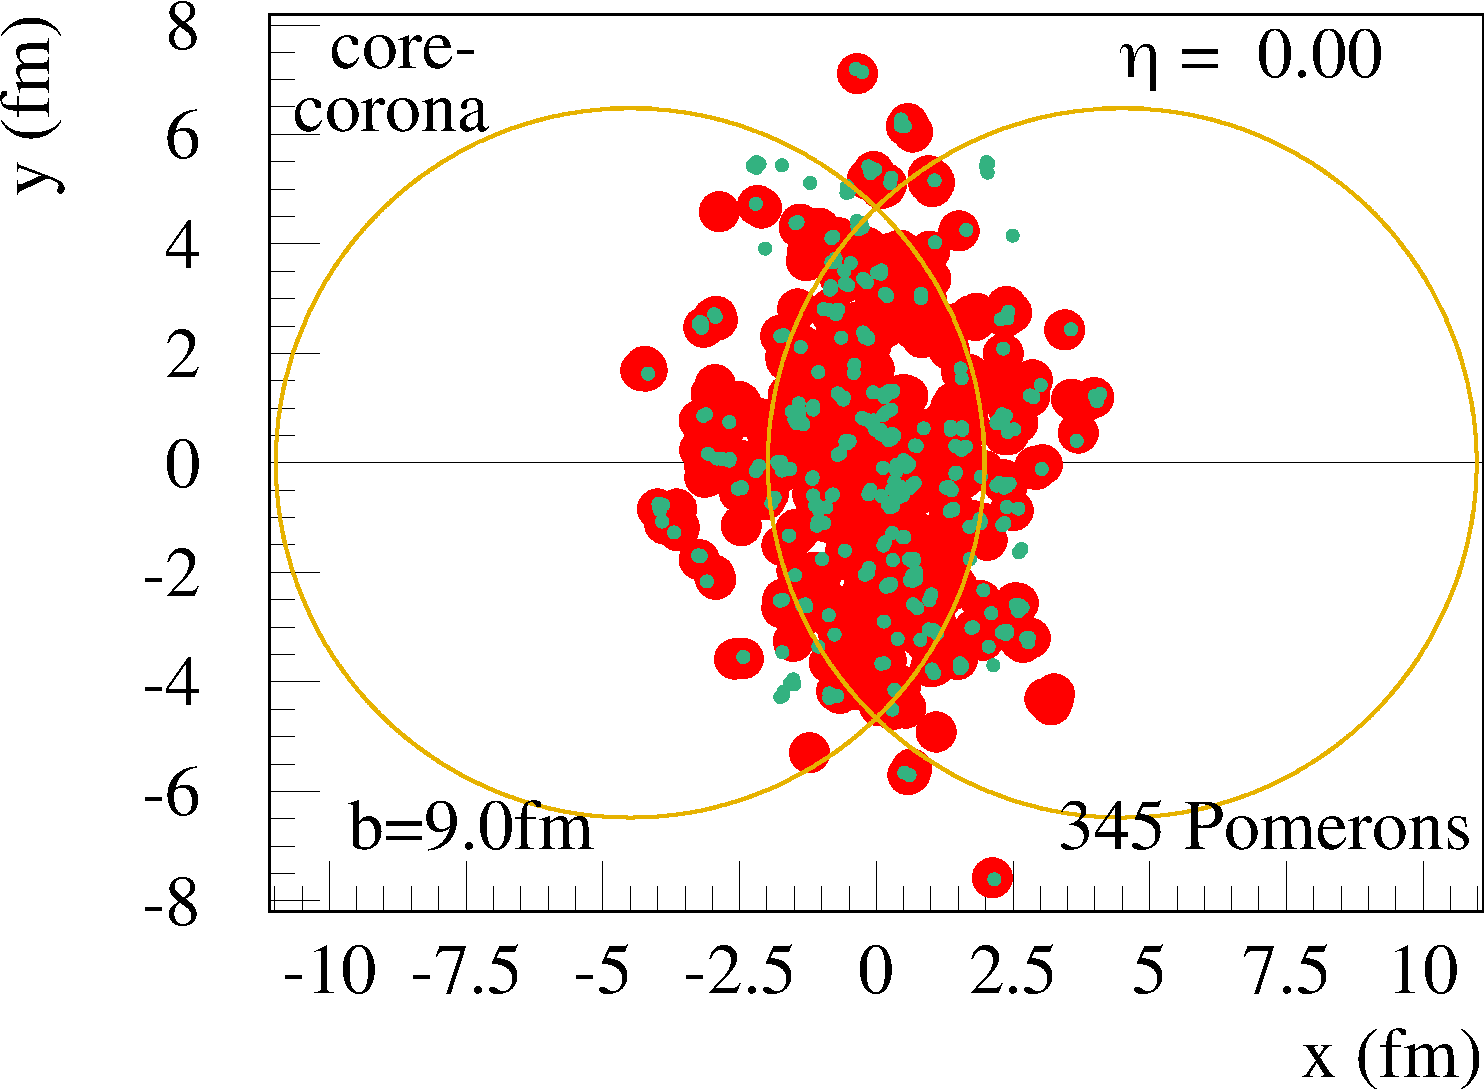
\includegraphics[width=.39\textwidth]{\imgpath/core1.pdf}}}\\
\subfloat[][]{\adjustbox{valign=m}{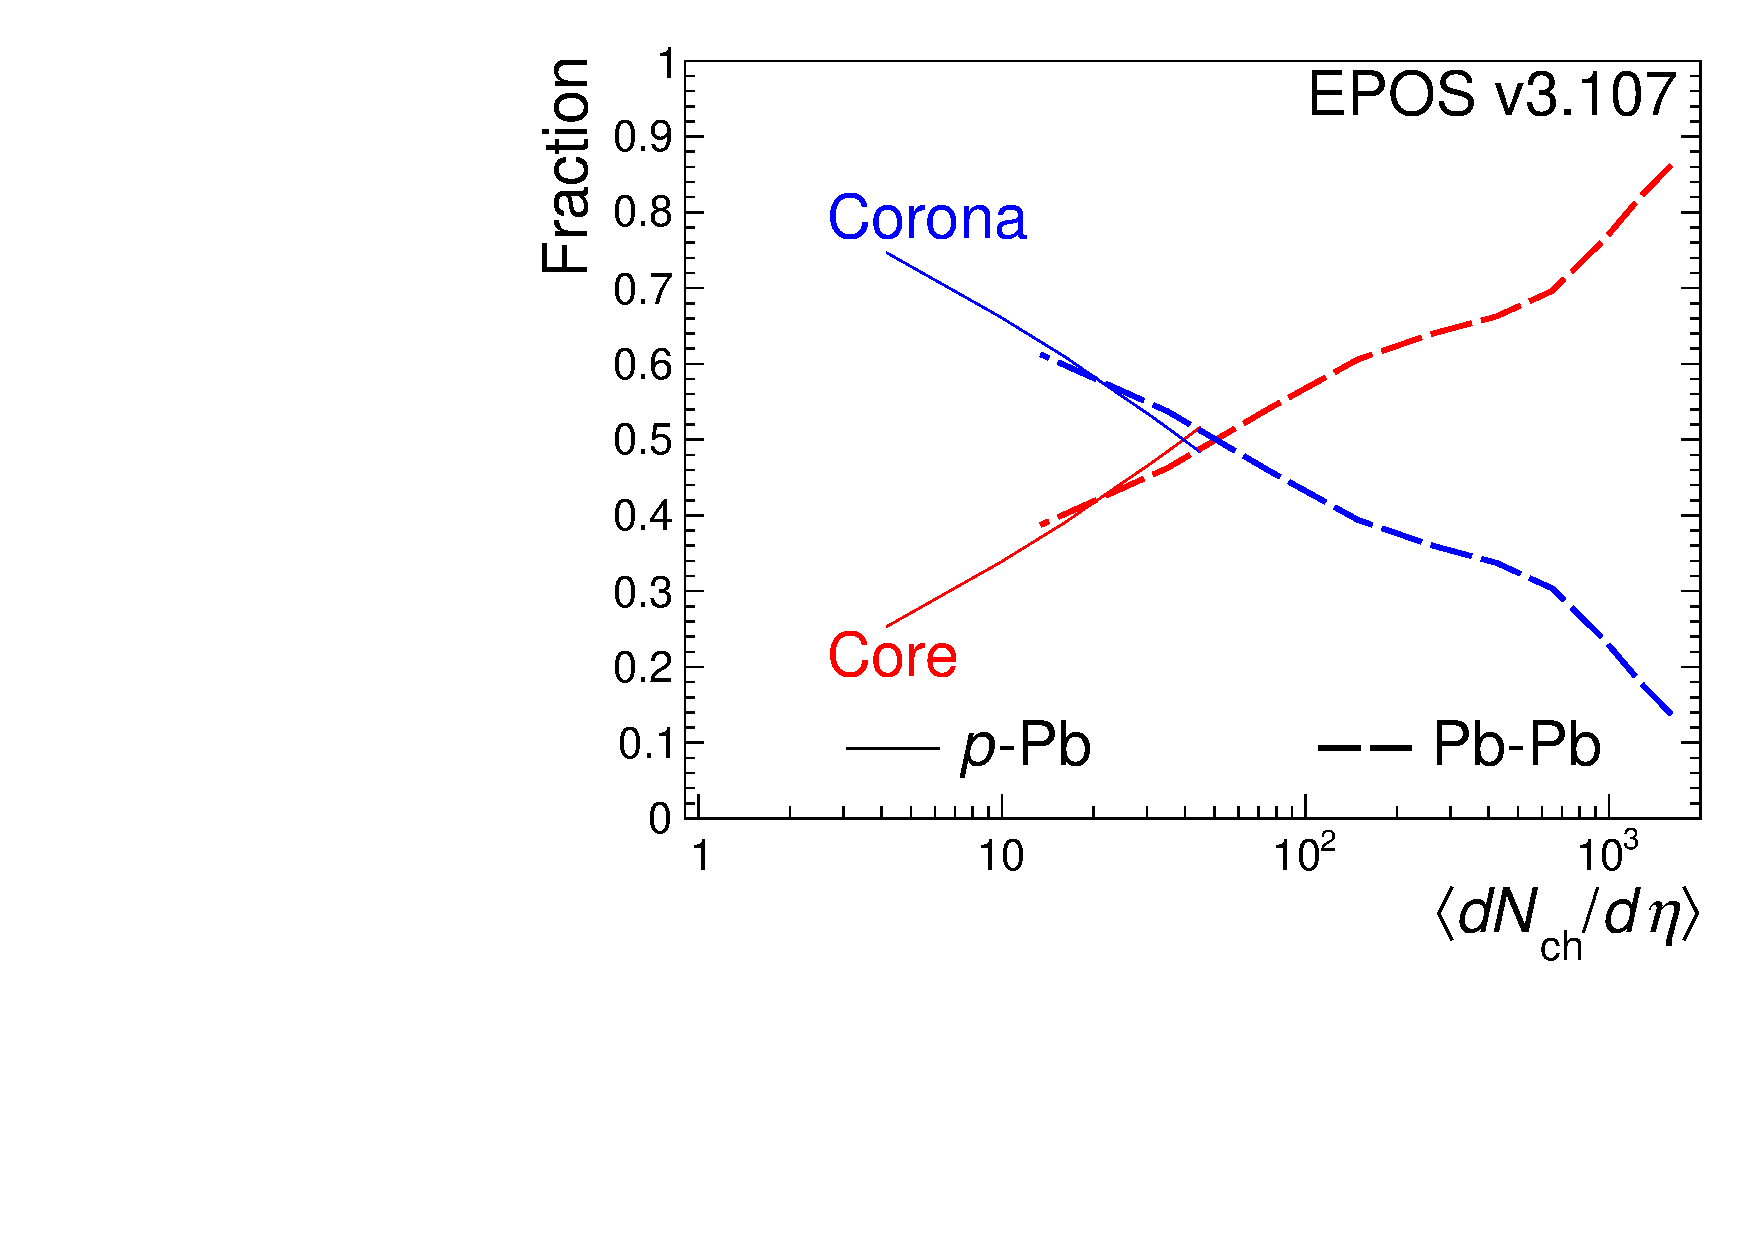
\includegraphics[width=.39\textwidth]{\imgpath/coco_ratio.pdf}}}
\caption{\textbf{(a)} Illustration of the partonic structure in the form of a parton ladder. \cite{pierogEPOSLHCTest2015} \textbf{(b)} Visualisation of the core (red) and corona (green) components in a peripheral $20-40\%$ collision of Pb-Pb with 345 initial multiple scatterings, modelled by EPOS3 \cite{knospeHadronicResonanceProduction2016} \textbf{(c)} Fractions of particle production associated with the core (red) and corona (blue) regions in p-Pb and Pb-Pb collisions, modelled by EPOS3. \cite{knospeHadronicResonanceProduction2021}}
\label{fig:colls:epos}
\end{figure}